\documentclass[12pt,openany]{book}

%PACKAGES%
\usepackage[inner=25.86mm, outer=18.24mm, top=25.86mm, bottom=33.48mm, papersize={154mm, 216mm}]{geometry}
\usepackage{graphicx}
\usepackage{fontspec}
\usepackage{enumitem}
\usepackage{sectsty}
\usepackage[]{titlesec}
\usepackage{verse}
\usepackage{fix-cm}%font size
\usepackage{multirow}%tables
\usepackage{array}%tables
\usepackage[hyphens]{url}
\usepackage{tocloft}
\usepackage{soulutf8}
\usepackage{marginnote}
\usepackage[english,main=dutch]{babel}
\usepackage[document]{ragged2e}
\usepackage{xcolor}
\usepackage{wrapfig}

\graphicspath{ {./images/} }

%this snippet of code is a bit of a hack to allow line break after em-dash (http://tex.stackexchange.com/questions/62800/lualatex-and-line-breaks-after-em-dashes)
\catcode`\—=13
\protected\def—{\unskip\textemdash\allowbreak}

%TABLE OF CONTENTS%
\renewcommand*{\cfttoctitlefont}{\Secfont\Large}%use tocloft
%TABLE OF CONTENTS%

%LINESPACE% SETS LINESPA\caps{ce}
\usepackage{setspace}
\setstretch{1.15}
%LINESPACE%

%FONTS% These are the normal SC fonts. We have a ``light'' skolar, too. 
\setmainfont[Numbers=OldStyle]{Alegreya HT Pro}
\setsansfont[Scale = MatchLowercase]{Alegreya Sans}
\setmonofont{Alegreya HT Pro}

\newfontfamily\Chapfont[ItalicFont=Alegreya Sans Italic]{Alegreya Sans}
\chapterfont{\Chapfont\LARGE\centering\mdseries\setstretch{1}}
\newfontfamily\Secfont[Numbers=OldStyle]{Alegreya Sans Medium}
\sectionfont{\Secfont\mdseries\large\setstretch{1}}

\hyphenpenalty=5000

%HEADER% 
\setlength{\headheight}{15pt}
\renewcommand{\chaptermark}[1]{\markboth{\thechapter.\ #1}{}}
\renewcommand{\sectionmark}[1]{\markright{\thesection\ #1}}

%HANGING LEFT%
\newcommand*{\vleftofline}[1]{\leavevmode\llap{#1}}
%HANGINGLEFT%

\definecolor{light-gray}{gray}{0.9}
\renewcommand\fbox{\fcolorbox{darkgray}{light-gray}}

\setlength{\fboxsep}{1em}

%WIDOWS & ORPHANS% 
\widowpenalty=10000
\clubpenalty=10000
%WIDOWS & ORPHANS%

%Applies various subtle improvements in typography. Use default.
\usepackage{microtype}
\frenchspacing

\usepackage[unicode, hidelinks, pdfauthor={Rainbodhi}, pdftitle={Verwelkom de regenboog}, pdfsubject={Boeddhisme}, pdfkeywords={Boeddhisme, LGBTIQA+, queer, transgender, lesbisch, homoseksueel, biseksueel, intersex, discriminatie}, pdfproducer={LuaTeX  beta-0.70.1}, pdfcreator={LaTeX2e}]{hyperref}

%DOCUMENT INFO. NOT USED IN TEXT.%
\title{Verwelkom de \protect\\ regenboog}
\author{Een gids om LGBTQIA+ te omarmen voor Boeddhisten}
\date{}
\begin{document}

\frontmatter

\newgeometry{margin=0px}

\begin{figure}[ht]
    \centering
    \makebox[0pt]{%
    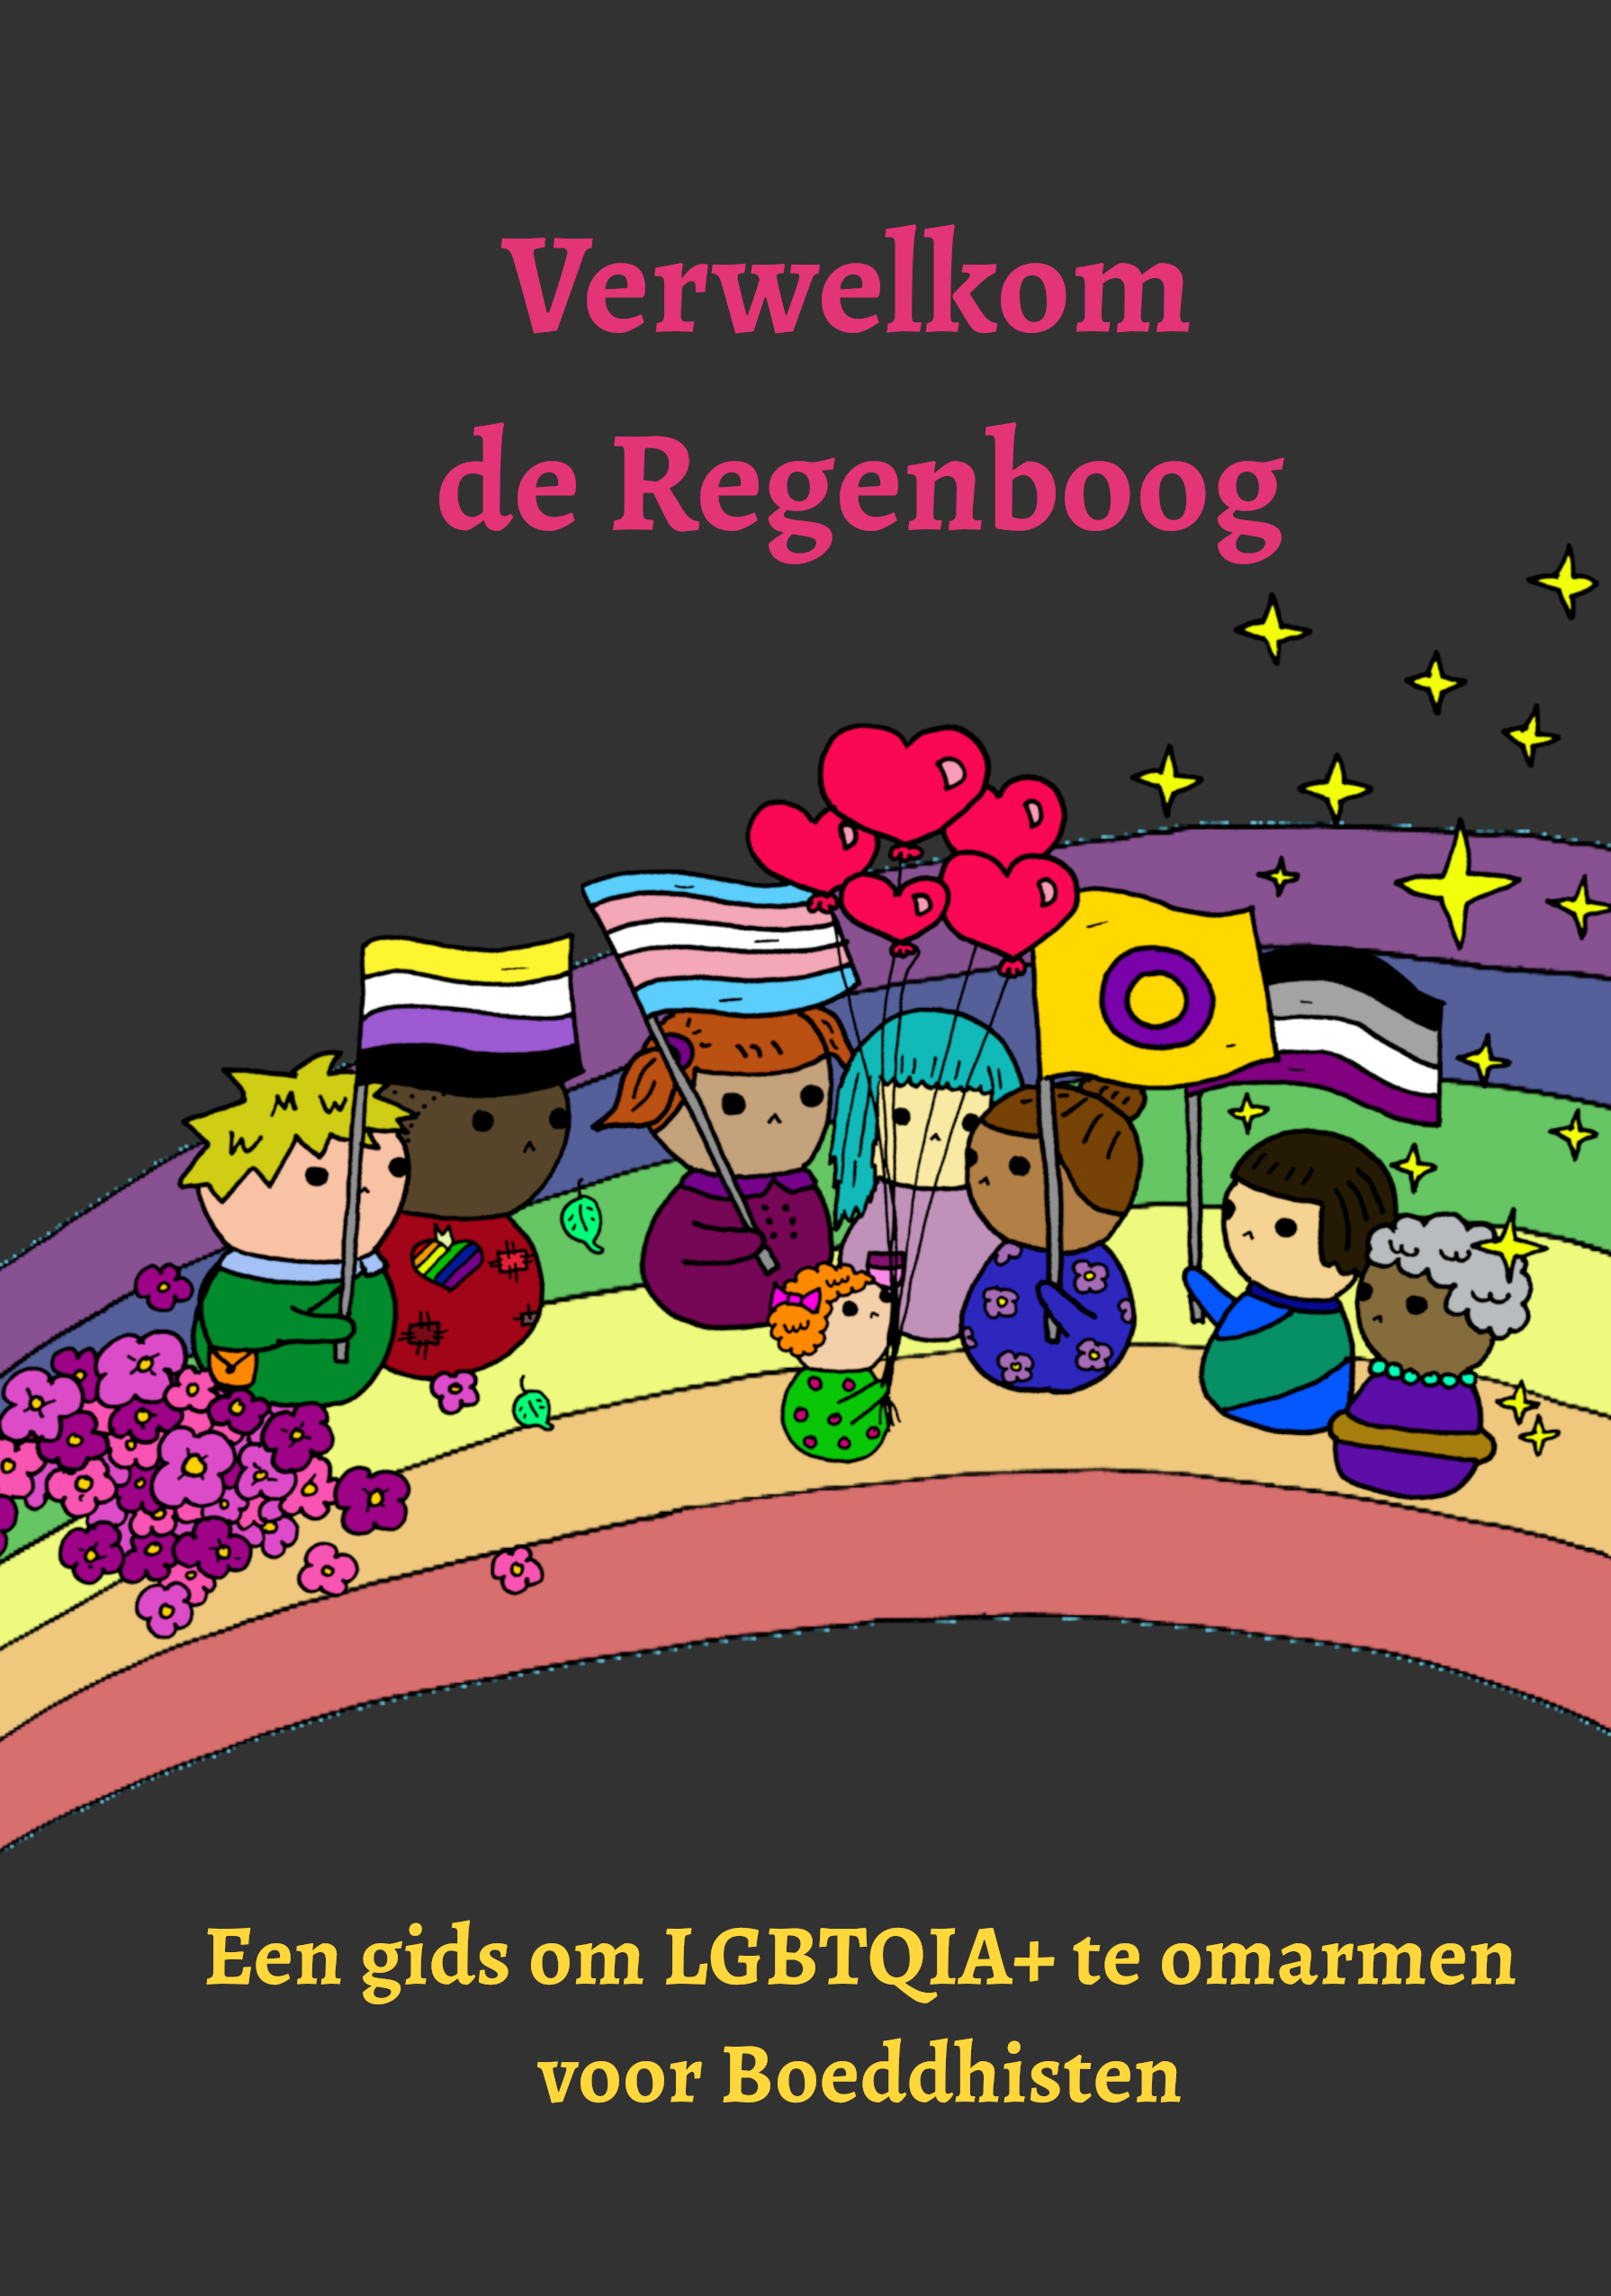
\includegraphics[width=\paperwidth]{front}}
\end{figure}

\restoregeometry

\begin{figure}[h]
    \makebox[150pt]{%
    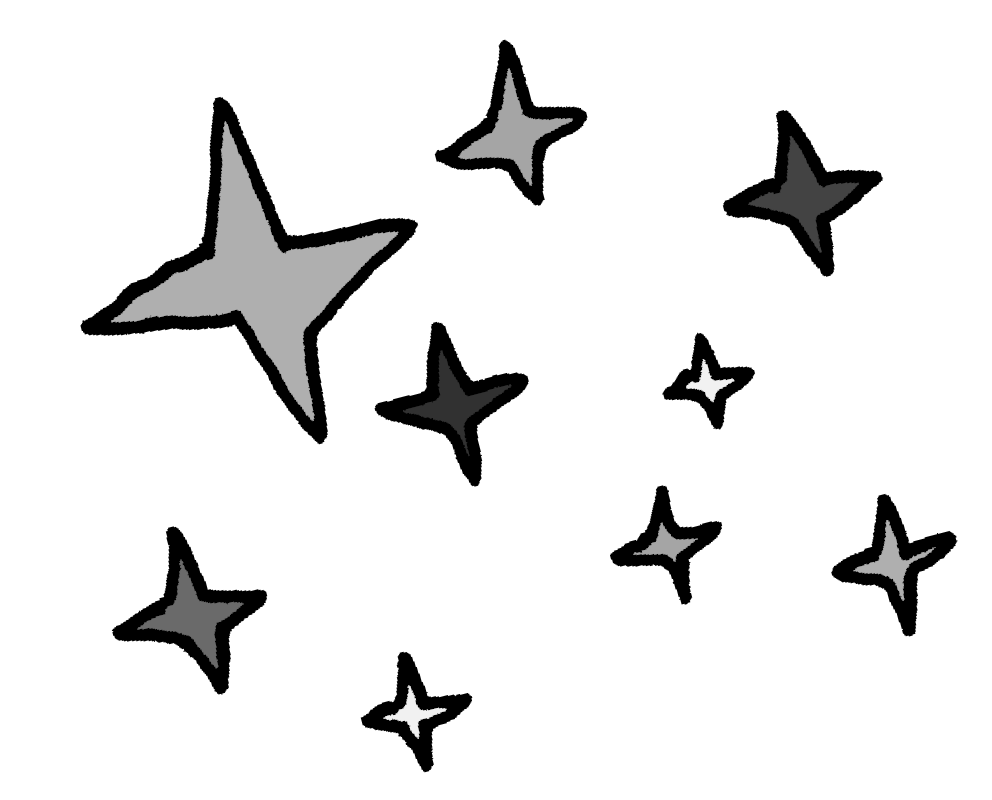
\includegraphics[width=0.4\paperwidth]{1bw.png}}
\end{figure}

\begin{center}

\thispagestyle{empty}

\sffamily

\caps{\Huge Verwelkom de Regenboog}

\medskip

\textit{ }

\caps{\LARGE Een Gids om LGBTQIA+ te Omarmen voor Boeddhisten}

\end{center}

\begin{figure}[h]
    \makebox[450pt]{%
    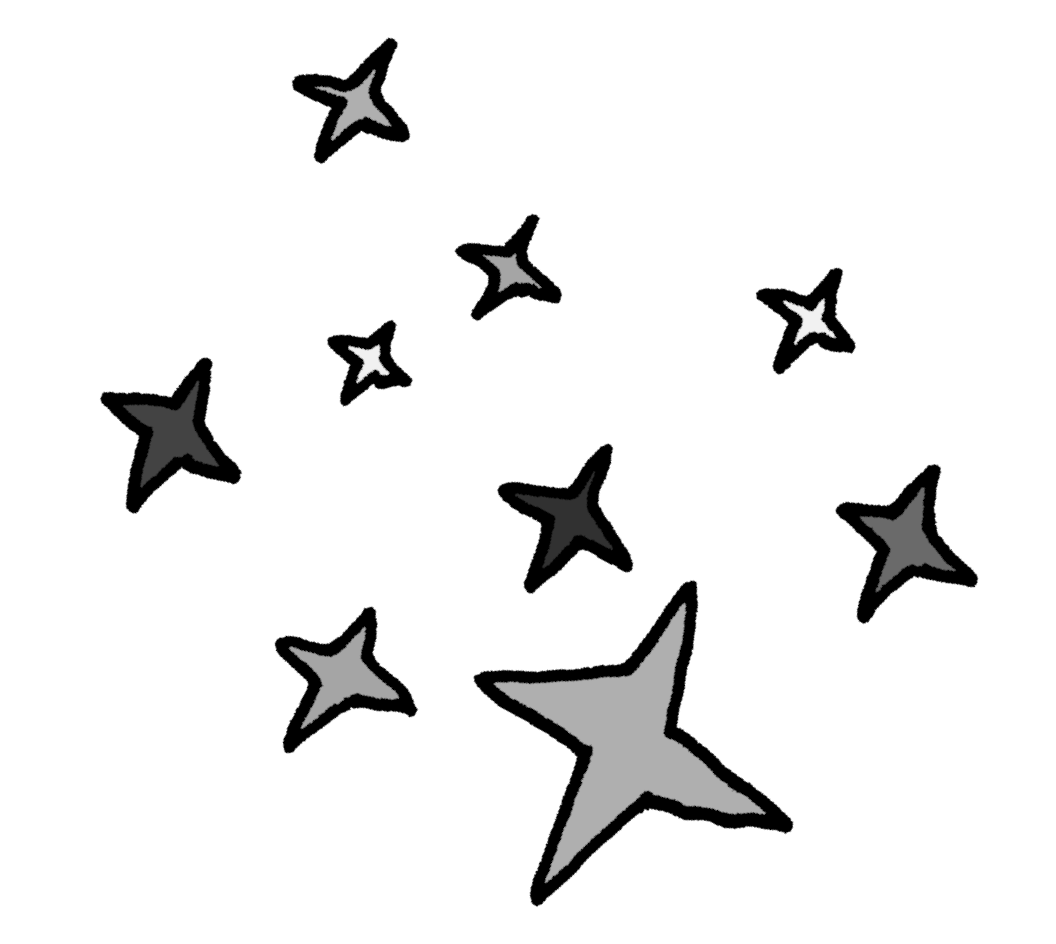
\includegraphics[width=0.4\paperwidth]{1bw2.png}}
\end{figure}

\newpage
\thispagestyle{empty}
\mbox

\newpage
\thispagestyle{empty}
\mbox

\tableofcontents
\thispagestyle{empty}
\markboth{}{}

\bigskip{}

\begin{figure}[h]
    \makebox[150pt]{%
    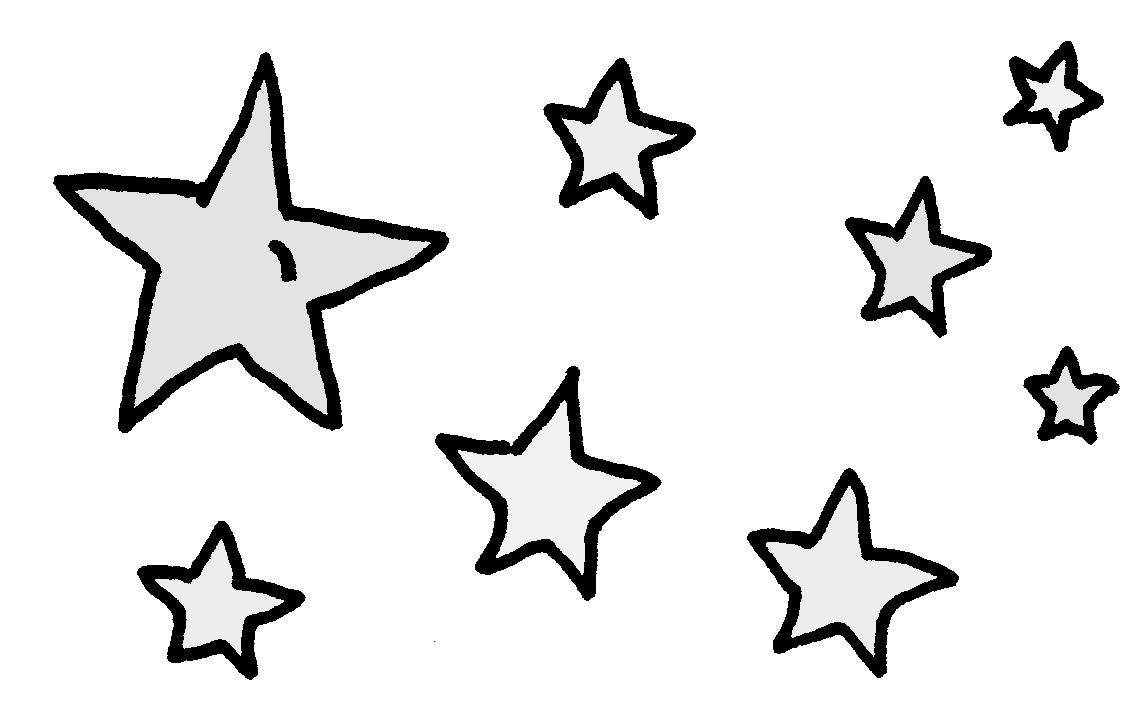
\includegraphics[width=0.4\paperwidth]{2bw.png}}
\end{figure}

\newpage
\thispagestyle{empty}

\rmfamily

\begin{center}\end{center}
\begin{center}

\vfill

\caps{\LARGE \textit{Moge Iedereen Gelukkig Zijn}}

\vfill

\end{center}

\begin{figure}[h]
    \centering
    \makebox[0pt]{%
    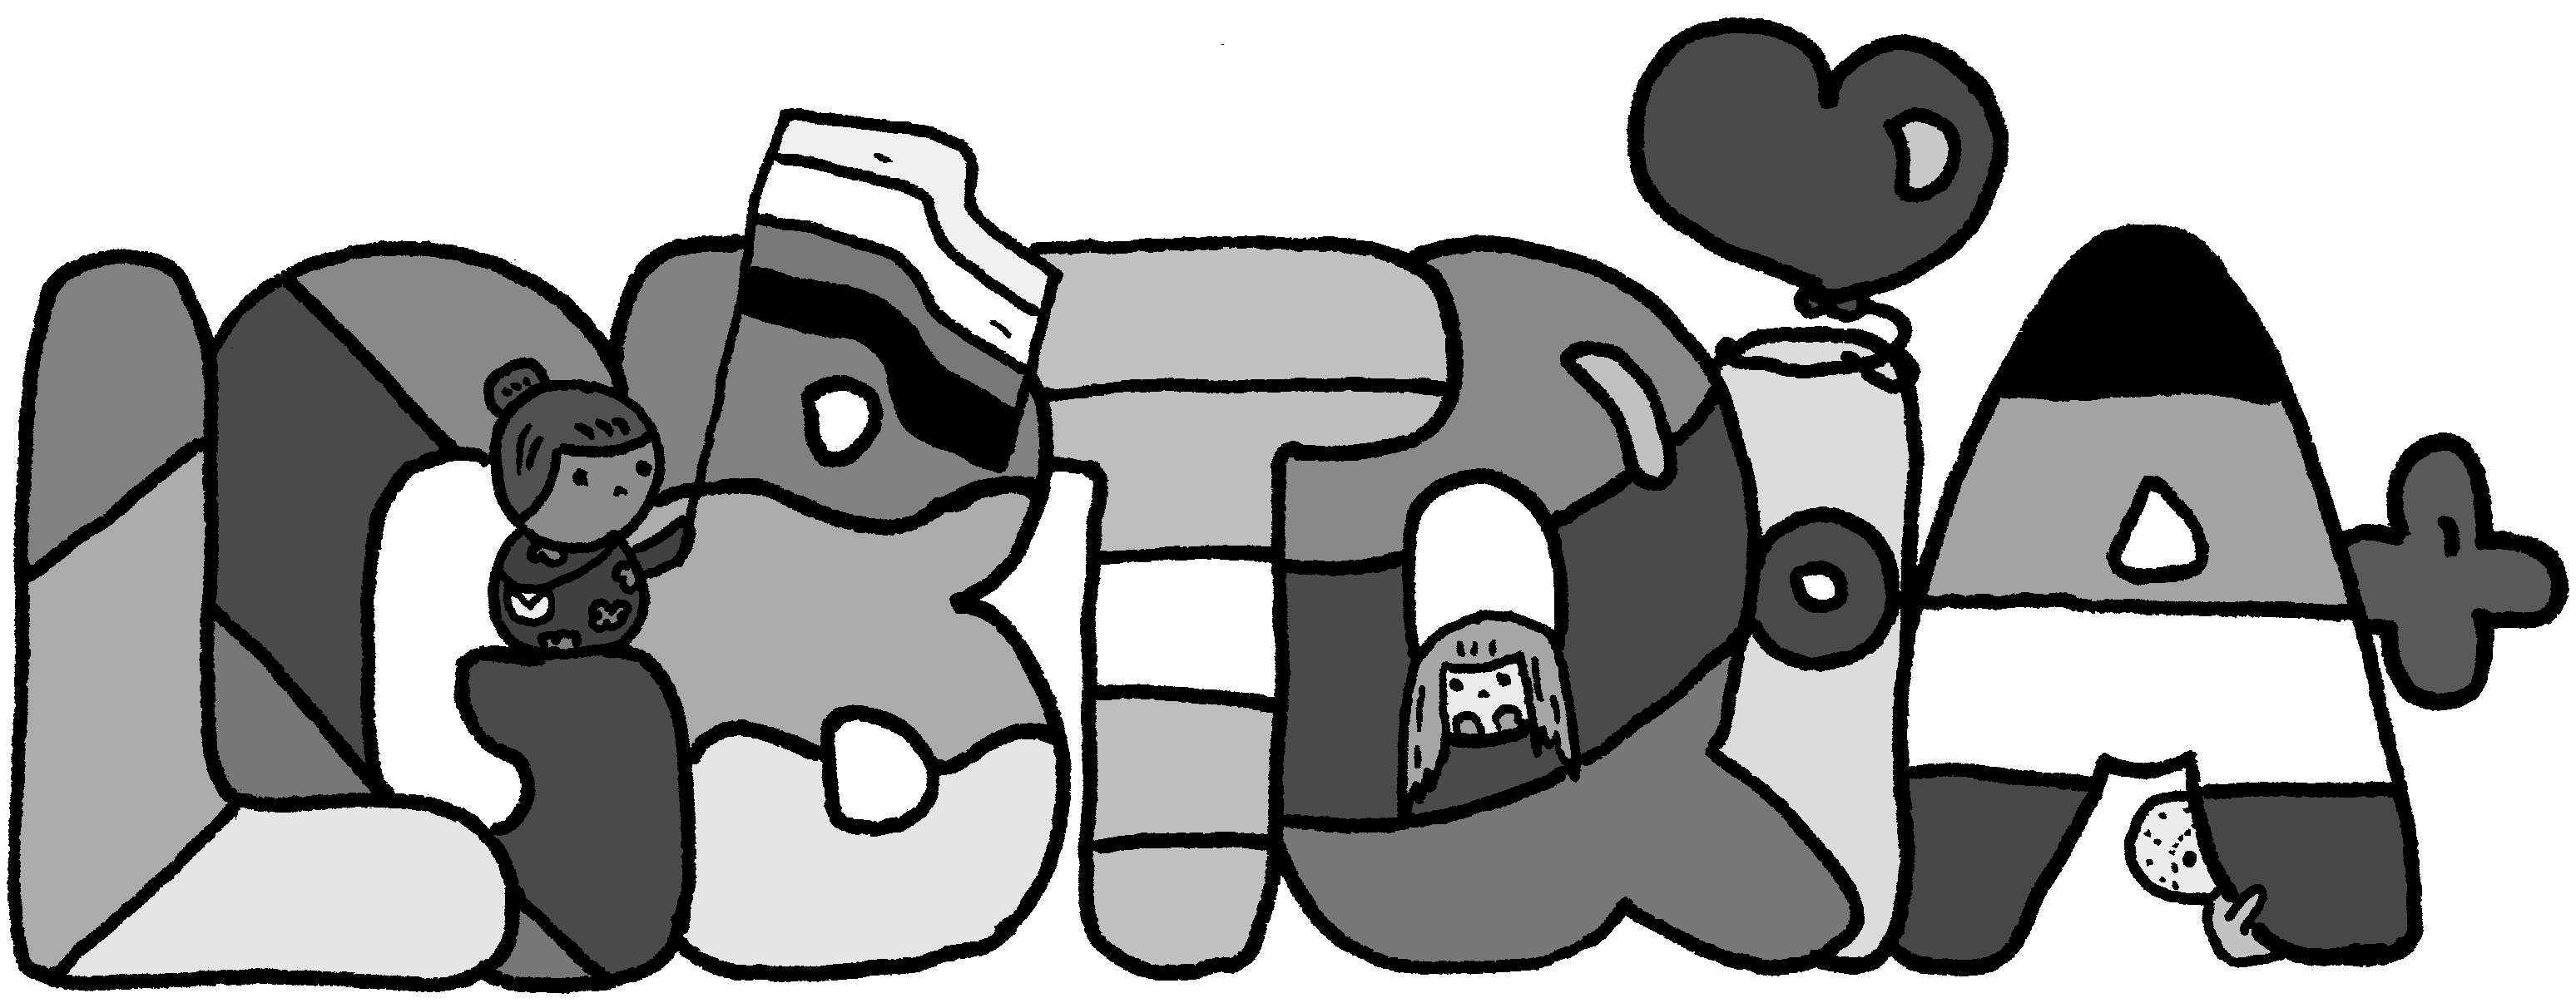
\includegraphics[width=0.8\paperwidth]{2-3bw.png}}
\end{figure}

\thispagestyle{empty}

\begin{figure}[h]
    \makebox[450pt]{%
    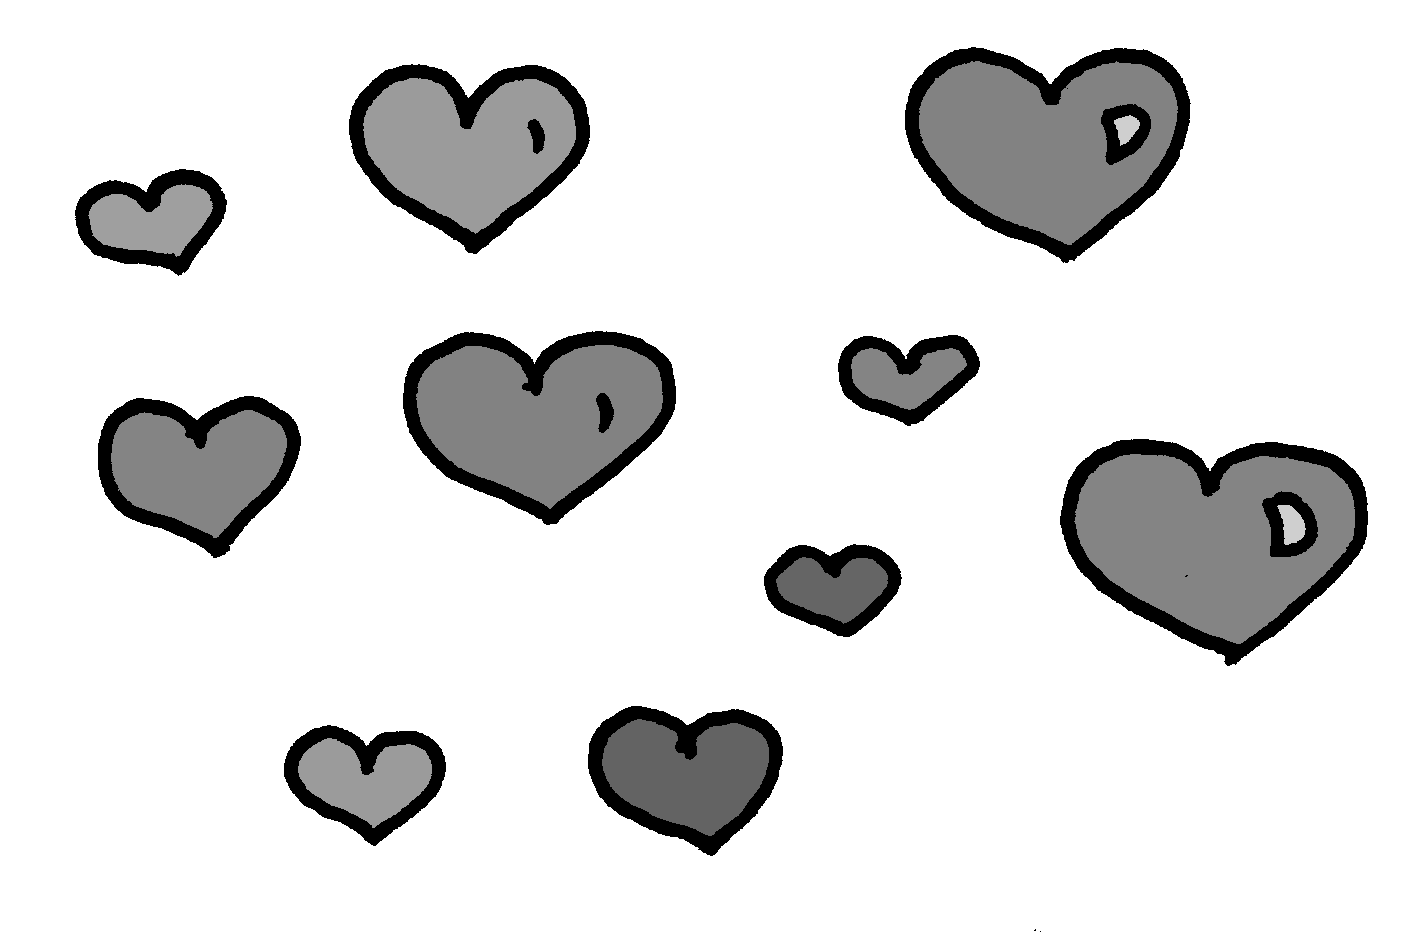
\includegraphics[width=0.4\paperwidth]{2bw2.png}}
\end{figure}

\thispagestyle{empty}

\mainmatter
\newpage
\thispagestyle{empty}
\begin{quote}
\centering
\textit{\Large Zolang individuen of boeddhistische organisaties zich schuldig maken aan homofobie, bifobie, transfobie of interfobie, houden zij haat, geweld en misbruik in stand.}
\end{quote}

\begin{figure}[h]
    \centering
    \makebox[0pt]{%
    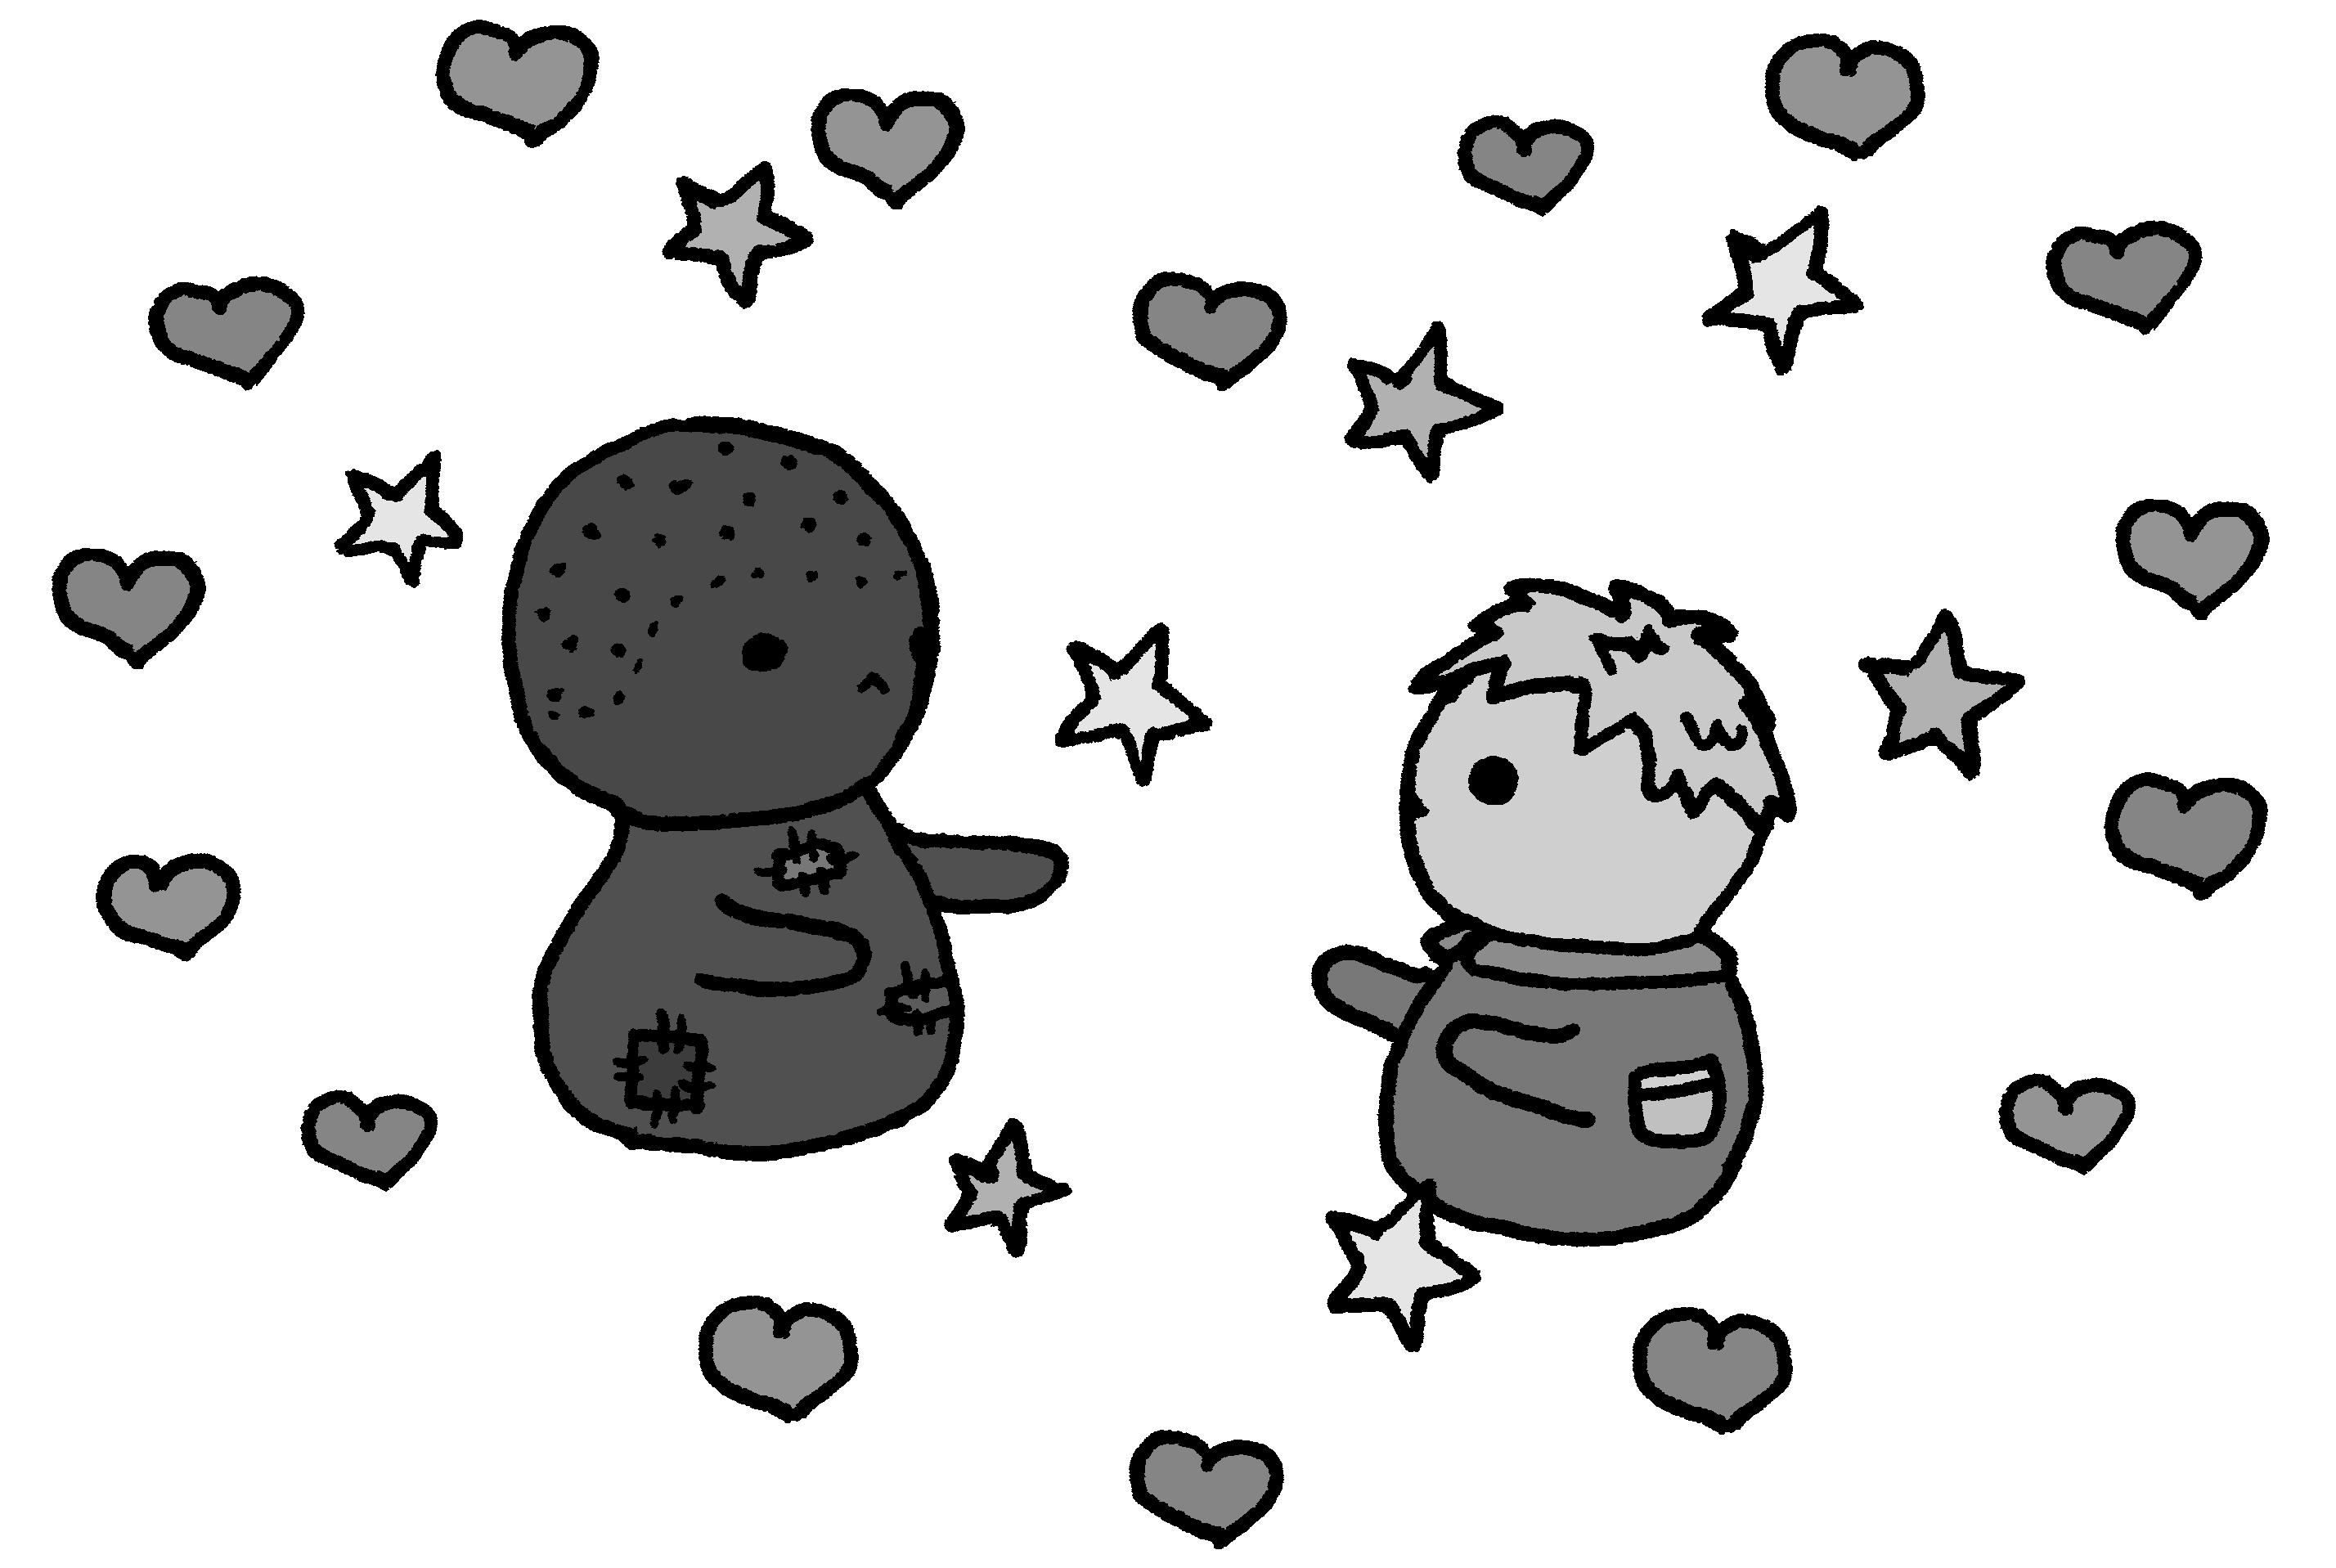
\includegraphics[width=0.8\paperwidth]{6-7bw.png}}
\end{figure}

\begin{quote}
\centering
\textit{\Large Als we inzicht krijgen in hoe er meer gastvrijheid en inclusiviteit kan zijn voor LGBTQIA+’ers, kunnen we echt liefdevolle vriendelijkheid beoefenen naar iedereen in onze gemeenschappen.}
\end{quote}

\setlength{\parindent}{15pt}
\chapter*{Verwelkom de regenboog}
\addcontentsline{toc}{chapter}{Verwelkom de regenboog}
\markboth{Verwelkom de regenboog}{Verwelkom de regenboog}

\begin{wrapfigure}{hl}{0.25\textwidth}
    \centering
    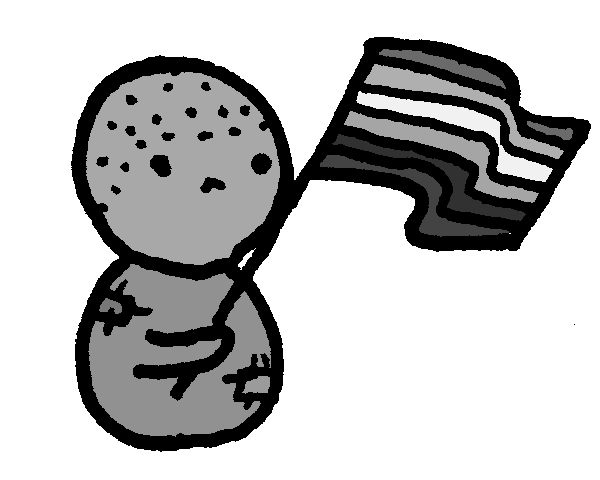
\includegraphics[width=0.25\textwidth]{2bw3.png}
\end{wrapfigure}
De boeddhistische LGBTQIA+ gemeenschap Rainbodhi heeft dit boekje gemaakt om  te helpen bij het veilig en gastvrij maken van boeddhistische tempels, kloosters en organisaties voor LGBTQIA+’ers, zodat die zich daar veilig en welkom kunnen voelen.

\begin{quote}
\textit{Samen kunnen we onze boeddhistische centra veiliger en meer inclusief maken voor de regenboog gemeenschap.}
\end{quote}

\phantomsection
\section*{Het regenboog acroniem}
\addcontentsline{toc}{section}{Het regenboog acroniem}

Het ‘LGBTQIA+’-acroniem staat voor lesbisch, gay (homoseksueel), biseksueel transgender, queer, intersekse en aseksueel. Het ‘+’ teken staat voor mogelijke andere identiteiten. We noemen dit het regenboog acroniem omdat de gemeenschap bestaat uit vele verschillende groepen, net als een regenboog bestaat uit vele verschillende kleuren. 

LGBTQIA+ beslaat een breed scala aan identiteiten. Denk aan fysieke kenmerken, seksuele geaardheid en genderidentiteiten. Deze groepen verschillen onderling behoorlijk, maar kunnen elkaar ook overlappen. Lesbisch, homoseksueel en biseksueel verwijst naar seksuele geaardheid; transgender verwijst naar een genderidentiteit; queer verwijst naar zowel genderidentiteit als seksualiteit; intersekse verwijst naar mensen geboren met zowel vrouwelijke als mannelijke fysieke kenmerken en aseksueel verwijst naar de afwezigheid van seksuele aantrekkingskracht. Combinaties van deze verschillende aspecten komen ook voor. 

Hoewel LGBTQIA+-identiteiten onderling verschillend zijn hebben ze allemaal te maken met dezelfde uitdagingen, zoals vooroordelen, discriminatie, juridische barrieres en geweld—alleen doordat ze zichzelf zijn.

\phantomsection
\section*{Samen werken aan verandering}
\addcontentsline{toc}{section}{Samen werken aan verandering}

LGBTQIA+’ers worden vaak geconfronteerd met afwijzing en onderdrukking door de samenleving en door religieuze gemeenschappen. De Boeddha  sprak zich vaak uit tegen discriminatie en zei dat alle levende wezens liefde verdienen, zonder uitzondering. Aangezien iedereen in staat is om verlichting te bereiken, zou het goed zijn als we niemand uitsluiten van onze boeddhistische gemeenschappen.  

Het is best mogelijk dat we ons niet eens realiseren dat onze boeddhistische organisaties, tempels en retraitecentra soms onwelkom aanvoelen voor LGBTQIA+’ers. Individuen begrijpen mogelijk niet dat hun acties en woorden schade kunnen brengen aan LGBTQIA+’ers. Organisaties zien misschien niet in hoe hun manier van doen en spreken LGBTQIA+’ers kwetst of uitsluit.  

Het goede nieuws is dat dit al aan het veranderen is en dat wij mee kunnen helpen.

\phantomsection
\section*{Horen wat er speelt binnen de gemeenschap}
\addcontentsline{toc}{section}{Horen wat er speelt binnen de gemeenschap}

Het is belangrijk om echt te luisteren naar LGBTQIA+-boeddhisten om te weten wat er speelt. Recent onderzoek, gesponsord door Rainbodhi en uitgevoerd door Dr. Stephen Kerry van de Charles Darwin Universiteit, wees uit dat Australische boeddhistische gemeenschappen best een uitdaging zijn voor LGBTQIA+-boeddhisten. Over hun eigen boeddhistische centra meldden respondenten:

\begin{itemize}
  \setlength\itemsep{0em}
  \item 61\% vond dat LGBTQIA+’ers verzwegen werden in boeddhistische centra en hun problemen werden genegeerd
  \item 55\% was soms terughoudend om hun LGBTQIA+-identiteit te onthullen
  \item 54\% had seksisme gezien of gehoord
  \item 37\% had homofobie gezien of gehoord
  \item 26\% had transfobie gezien of gehoord
  \item 26\% had racisme gezien of gehoord
  \item 16\% had te horen gekregen dat hun LGBTQIA+-identiteit niet overeenkomt met de boeddhistische leer.
\end{itemize}

\begin{wrapfigure}{l}{0.15\textwidth}
    \centering
    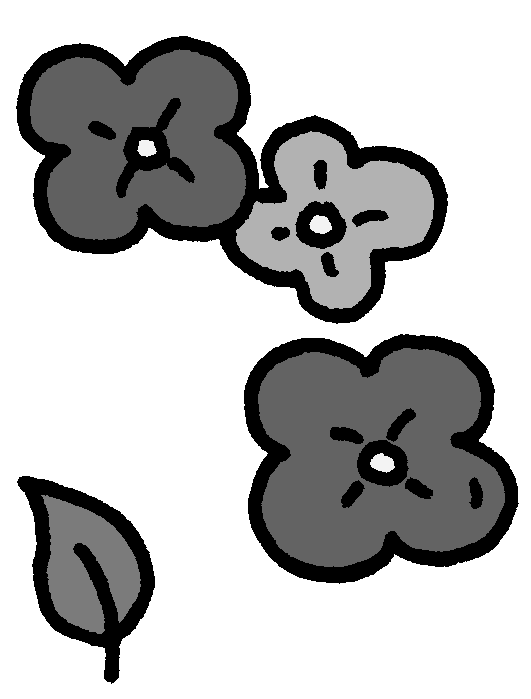
\includegraphics[width=0.15\textwidth]{2bw4.png}
\end{wrapfigure}

Deze resultaten laten zien dat boeddhistische centra nog niet altijd een veilige plek zijn voor LGBTQIA+-boeddhisten. Het erkennen dat er vooroordelen en discriminatie bestaan binnen de boeddhistische centra is een belangrijke eerste stap om het nodige te kunnen veranderen qua veiligheid en inclusie.

\phantomsection
\section*{Boeddhisme heeft LGBTQIA+-geschiedenis (en toekomst)}
\addcontentsline{toc}{section}{Boeddhisme heeft LGBTQIA+-gechiedenis (en toekomst)}

Er zijn in het verleden altijd queer, trans en intersekse mensen geweest en onder de LGBTQIA+’ers zijn ook spirituele mensen, dus is het niet verwonderlijk dat het boeddhisme een LGBTQIA+-geschiedenis heeft.

In oude boeddhistische teksten wordt zonder enig gevoel voor moreel oordeel of negativiteit gesproken over aantrekking tot, en seksualiteit met het zelfde geslacht. Er zijn ook verslagen van kloosterlingen die wisselden tussen het ene en het andere gender. De oude Indiase samenleving erkende een categorie mensen die noch als man, noch als vrouw werd gezien (deze zouden we tegenwoordig wellicht transgender of het derde gender noemen) en noemden ook een andere categorie mensen met zowel mannelijke als vrouwelijke geslachtskenmerken (die wij wellicht intersekse zouden noemen). In de boeddhistische geschiedenis werden deze groepen al sociaal benadeeld en gestigmatiseerd. Voor sommige groepen duurt deze discriminatie tot op de dag van vandaag nog voort.

\subsubsection*{Pride in het boeddhisme}

LGBTQIA+'ers hebben als kloosterlingen, lekenvolgers, leraren en geleerden hun bijdrage geleverd aan het opbloeien van het boeddhisme. Hun verhalen worden helaas vaak vergeten of hun ervaringen doodgezwegen. Tegenwoordig is er steeds meer acceptatie en begrip voor LGBTQIA+’ers in het algemeen en dus is de tijd rijp dat ook de boeddhistische organisaties de regenbooggemeenschap omarmen en zinvol gaan steunen. Hierdoor zullen LGBTQIA+’ers in de toekomst vaker als gewaardeerde leden van onze boeddhistische gemeenschappen worden gerekend.

\begin{quote}
\textit{Iedereen, ongeacht gender of seksuele voorkeur, verdient het om vrij van angst voor afwijzing te leven en om trots te zijn op zichzelf.}
\end{quote}

\begin{figure}[h]
    \centering
    \makebox[0pt]{%
    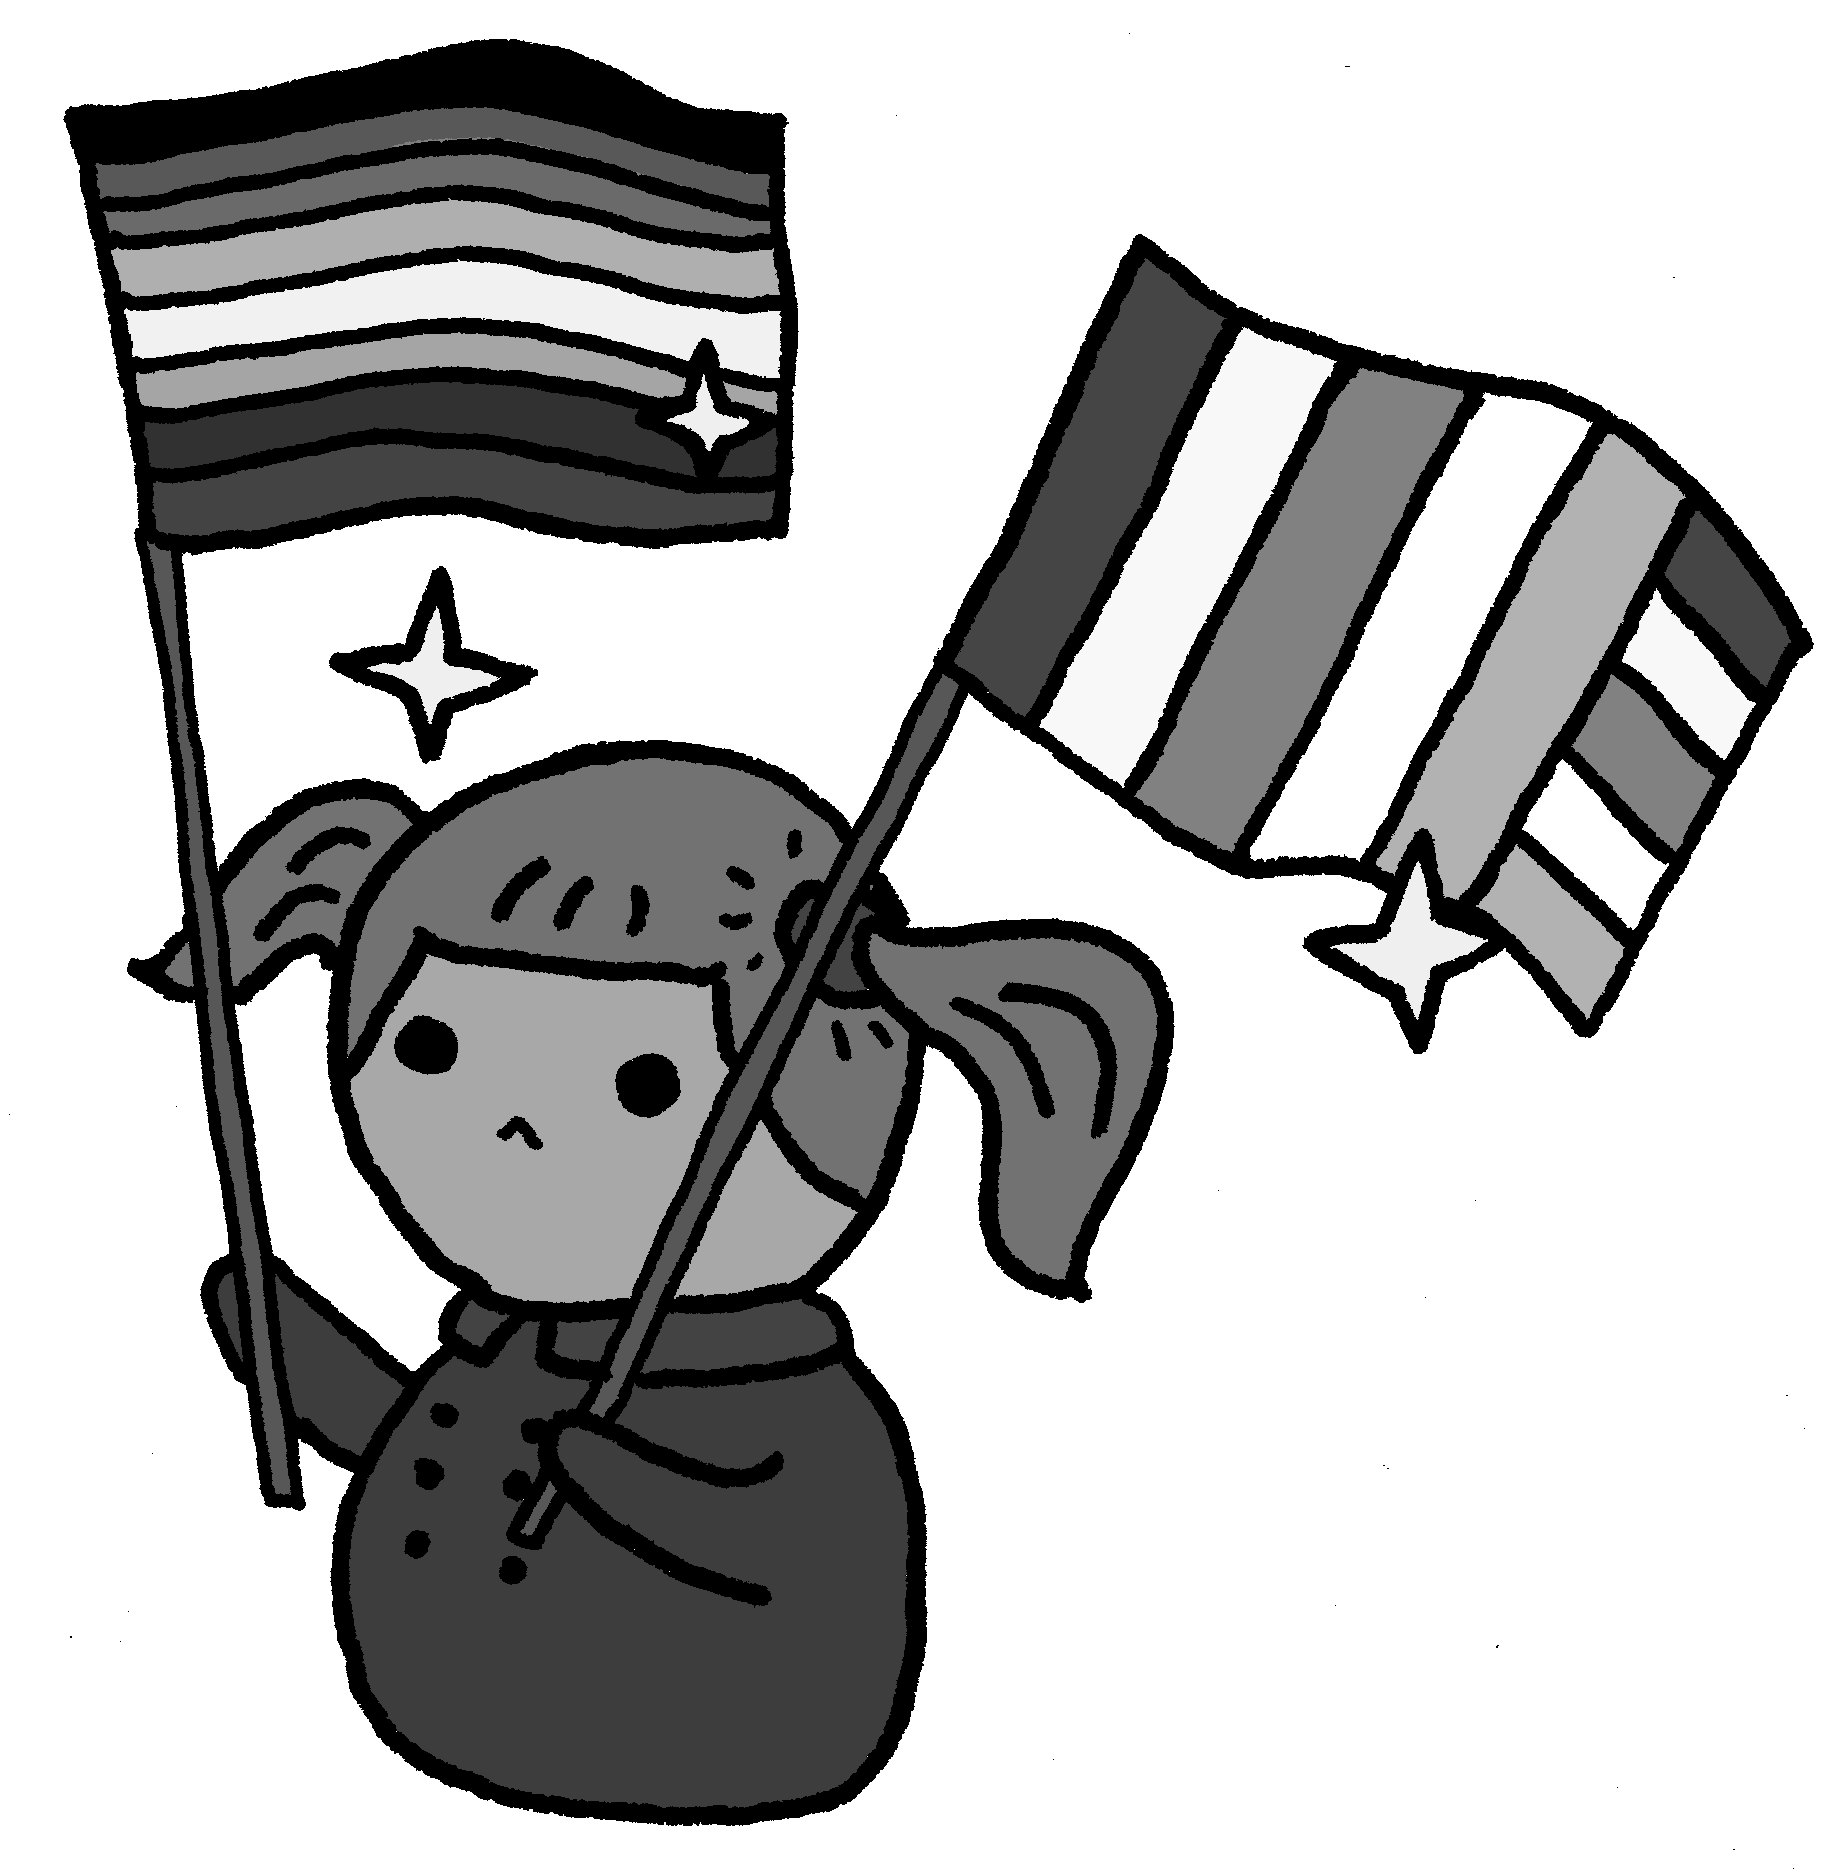
\includegraphics[width=0.3\paperwidth]{9bw.png}}
\end{figure}

\newpage
\thispagestyle{empty}

\bigskip

\bigskip

\begin{figure}[h]
    \centering
    \makebox[0pt]{%
    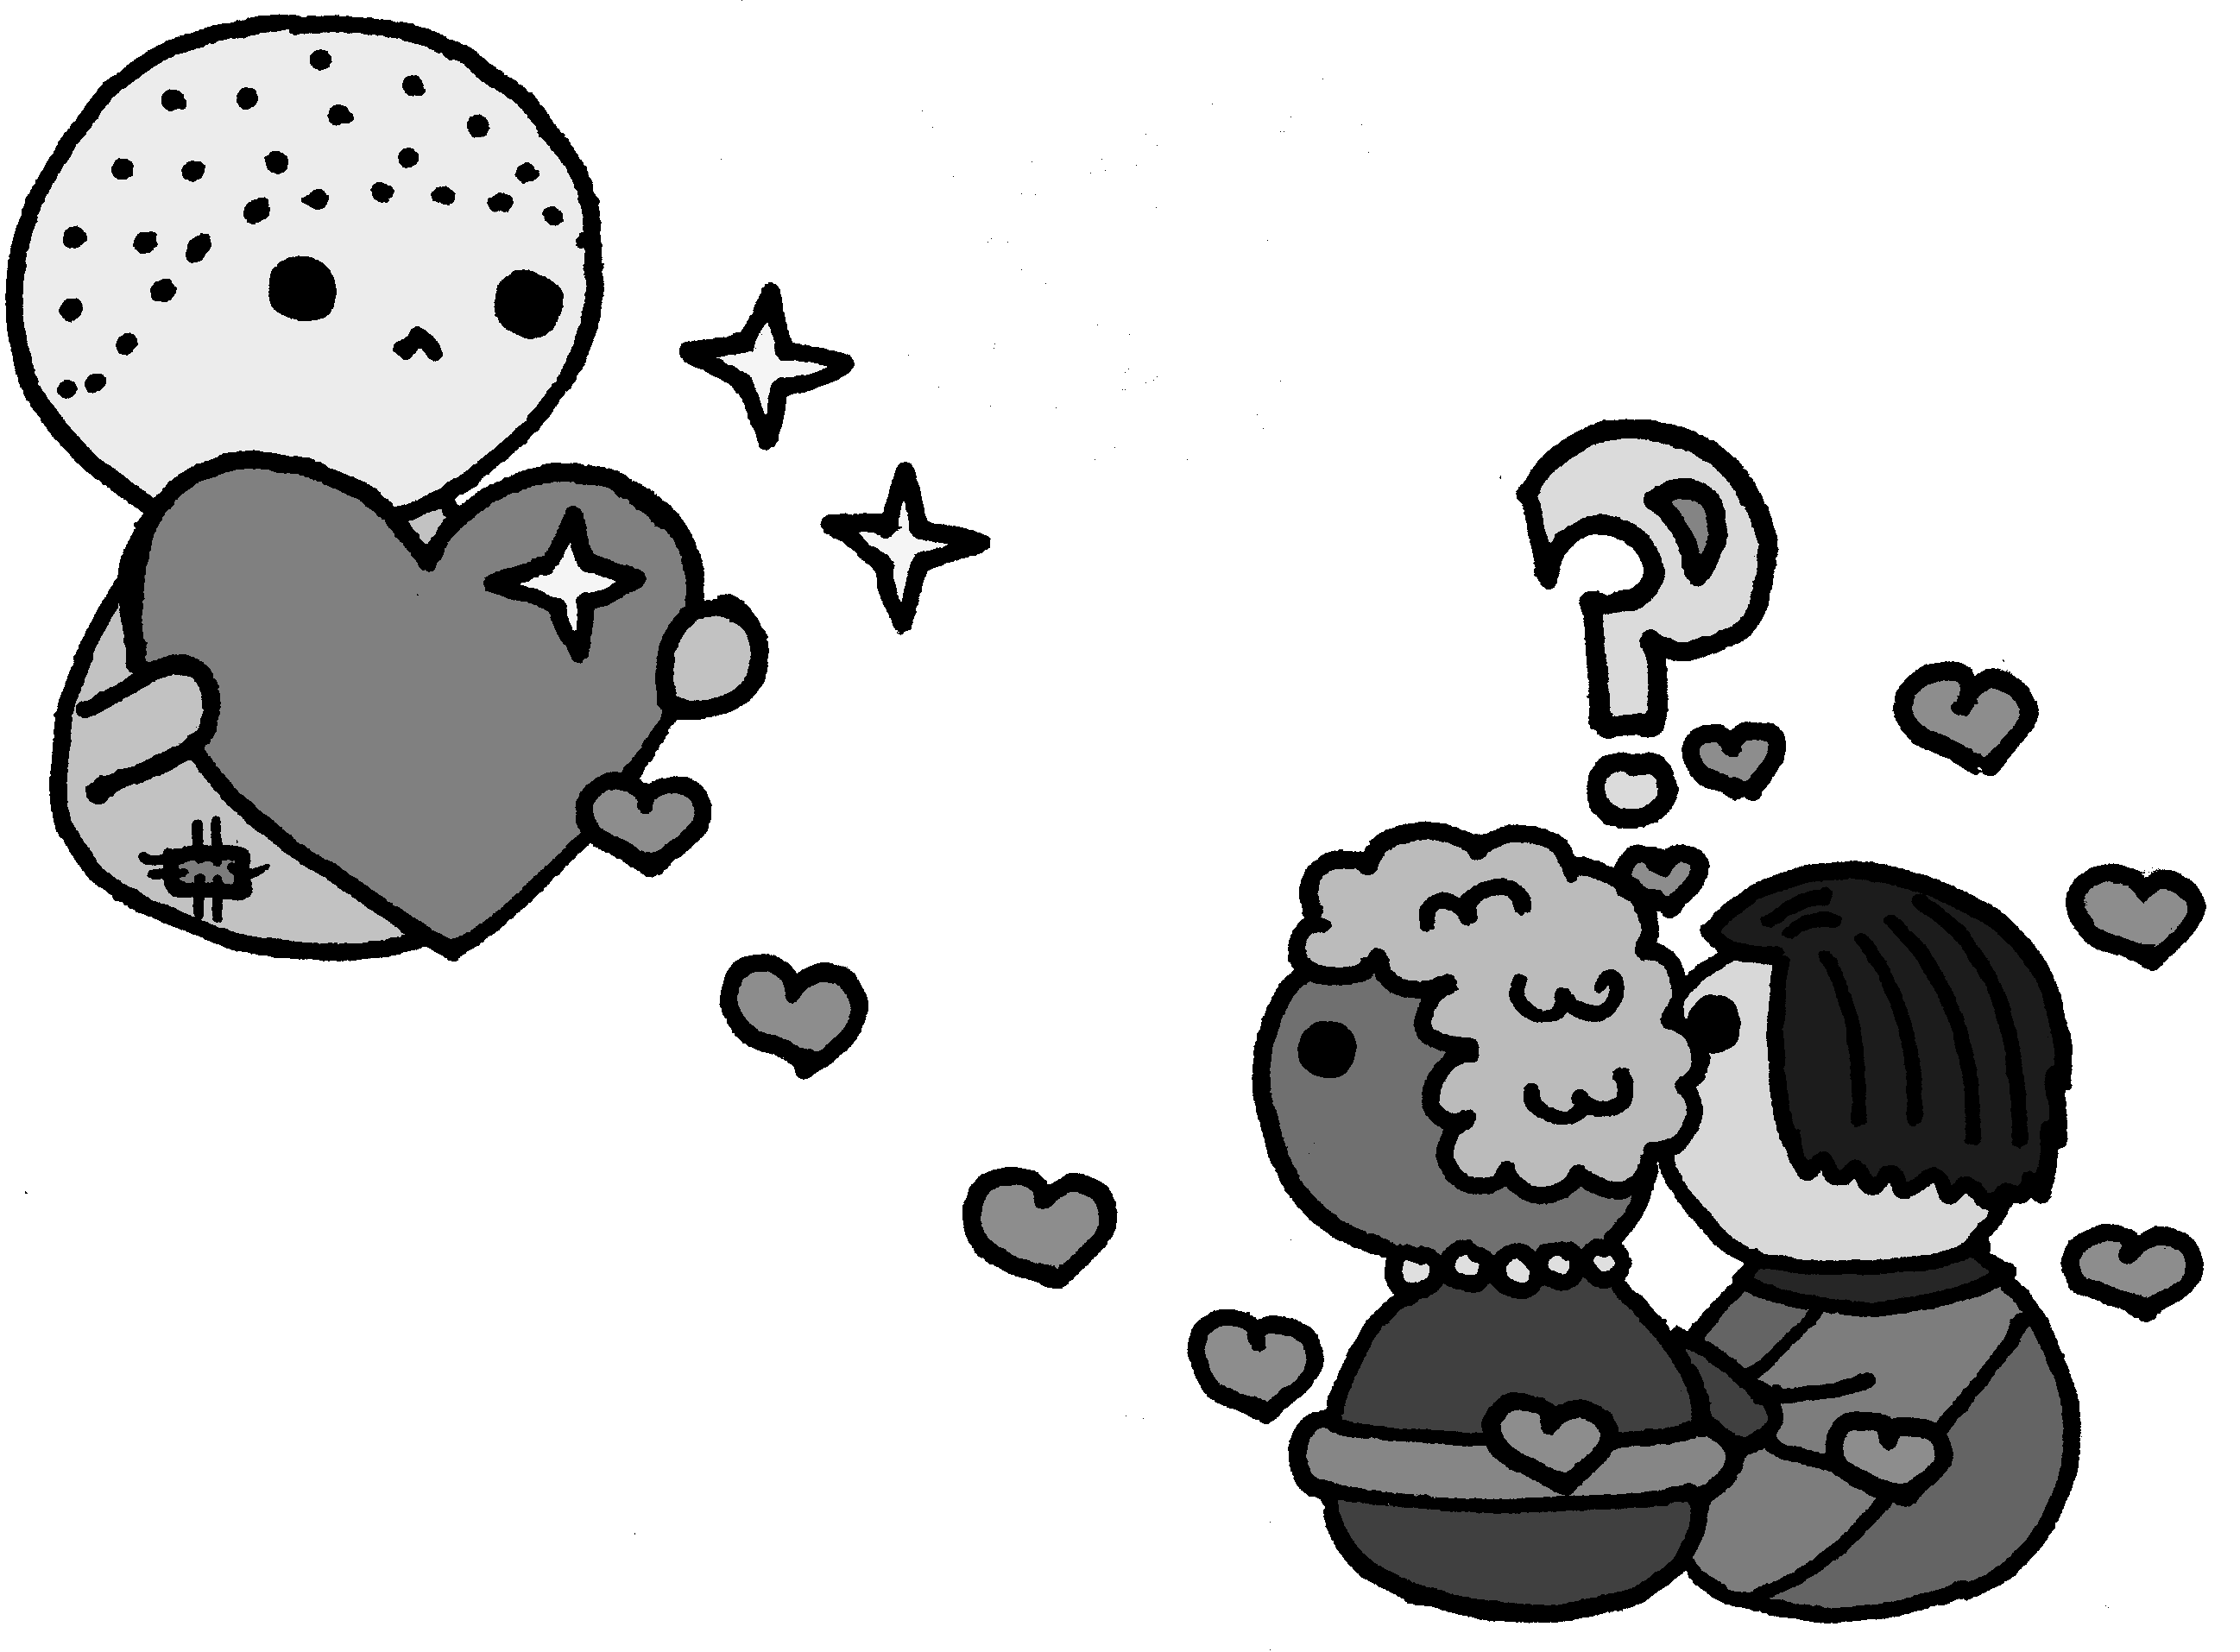
\includegraphics[width=0.7\paperwidth]{10bw.png}}
\end{figure}

\begin{quote}
\centering
\textit{\Large Ware vriendschap beslaat het geheel van het spirituele pad.}
\end{quote}

\chapter*{Wees een spirituele vriend van LGBTQIA+-boeddhisten}
\addcontentsline{toc}{chapter}{Wees een spirituele vriend van LGBTQIA+-boeddhisten}
\markboth{Verwelkom de regenboog}{Wees een spirituele vriend van LGBTQIA+-boeddhisten}

\phantomsection
\section*{Wees een bondgenoot}
\addcontentsline{toc}{section}{Wees een bondgenoot}

Een spirituele vriend zijn is een belangrijk onderdeel van het boeddhisme. Door een LGBTQIA+ bondgenoot te zijn, kun je anderen een veilig en welkom gevoel geven.

Een  bondgenoot steunt de burgerrechten van LGBTQIA+’ers en is actief in het bestrijden van homofobie, bifobie, transfobie en interfobie. Bondgenoten zijn vaak heteroseksueel en/of cisgender (mensen die zich identificeren met het geslacht dat ze bij geboorte toegewezen kregen). Bondgenoten beseffen dat ze het voorrecht hebben dat ze niet tegen dezelfde sociale hindernissen aan hoeven te lopen als LGBTQIA+’ers en dus gebruiken ze deze voorrechtpositie om discriminatie van deze gemeenschap tegen te gaan. 

Een bondgenoot kan iemand zijn die zich identificeert met de LGBTQIA+-gemeenschap en een groep ondersteunt waarmee die zichzelf niet identificeert. Een cisgender homoseksuele man kan bijvoorbeeld bondgenoot zijn voor transgender mensen. Een intersekse person kan opkomen voor de rechten van mensen die op hetzelfde geslacht vallen.

Bondgenoten nemen de taak op zich om uit te leggen tegen welke problemen LGBTQIA+’ers in de wereld aan lopen. Om een goede bondgenoot te zijn, is het ten eerste belangrijk om te luisteren naar LGBTQIA+’ers en te leren over hun uiteenlopende ervaringen. Dit betekent basiskennis, zoals wat de letters in het acroniem betekenen, het verschil tussen seksualiteit en gender, hoe de problemen van transgender mensen verschillen van die van LGB’ers, en welke mensenrechten intersekse mensen willen verwerven.
\begin{wrapfigure}{hr}{0.25\textwidth}
    \centering
    
\includegraphics[width=0.25\textwidth]{12bw.png}
\end{wrapfigure}

\begin{quote}
\textit{Een bondgenoot zijn is een bewijs van vriendschap en mededogen}
\end{quote}

\phantomsection
\section*{Inclusie bevorderen}
\addcontentsline{toc}{section}{Inclusie bevorderen}

Het is goed om te beseffen dat er LGBTQIA+’ers in boeddhistische gemeenschappen zijn. Je kunt er nooit vanuit gaan dat iedereen heteroseksueel is, of dat we door naar iemand te kijken meteen weten van welk geslacht/gender iemand is of welke voornaamwoorden gepast zijn. Erkennen dat ook LGBTQIA+’ers onze tempels, retraites en centra bezoeken is de eerste stap om meer inclusief te zijn.

LGBTQIA+’ers hebben zich vaak gedwongen gevoeld om onzichtbaar te blijven in boeddhistische gemeenschappen en hadden vaak het gevoel dat hun specifieke behoeften niet werden gezien, laat staan dat erin werd voorzien.  Het is niet voor iedereen makkelijk om open te zijn over hun identiteit vanwege de angst om afgewezen te worden. Het kan ongemakkelijk voelen om te praten over kwesties die hen aangaan. Het zou kunnen dat ze zich onzeker voelen over hun veiligheid binnen de boeddhistische gemeenschap doordat ze in het verleden een slechte ervaring hebben gehad bij een ander boeddhistisch centrum of religie in het algemeen. We kunnen onze goede wil en spirituele vriendschap tonen door LGBTQIA+’ers te laten weten dat ze welkom zijn in onze gemeenschappen.

\subsubsection*{Inclusie betekent veranderingen aanbrengen}

Het verwelkomen van LGBTQIA+ers’ is een mooi begin, maar echte inclusie betekent het wegnemen van bestaande barrieres die mensen uitsluiten. Includeren vraagt om werkelijk inzicht in het perspectief van LGBTQIA+’ers. In de praktijk kan dit betekenen dat het nodig is om de administratie onder de loep te nemen. Het aanpassen van lidmaatschaps- en registratieformulieren bijvoorbeeld, waar vaak alleen mannelijke of vrouwelijke opties op staan. of het maken van fysieke veranderingen, zoals het aanbieden van genderneutrale toiletten en verblijfsopties.  Verandering kan ook op persoonlijk niveau: door meer bewust om te gaan met woordkeuze en welke vragen nodig zijn op formulieren zodat LGBTQIA+’ers niet het gevoel krijgen er niet bij te horen.

Boeddhistische centra zouden een beleid moeten hebben over inclusiviteit zodat iedereen zich welkom kan voelen. Om dit inclusieve beleid veilig te stellen moeten de procedures openbaar zijn zodat er op toegezien kan worden dat iedereen veilig en welkom is. Het moet bekend zijn welke wegen bewandeld kunnen worden om een eventueel probleem op te kunnen lossen.

\phantomsection
\section*{Vier diversiteit} 
\addcontentsline{toc}{section}{Vier diversiteit}

Er zijn veel manieren om de regenbooggemeenschap te steunen als boeddhist en boeddhistische organisatie. Een positieve houding ten aanzien van diversiteit is een uitgesproken kans om “empathische vreugde” te voelen en het geluk van anderen te bevorderen.

\begin{itemize}
  \setlength\itemsep{0em}
  \item Doe met je hele organisatie een LGBTQIA+ diversiteits- en inclusietraining. Moedig andere boeddhistische organisaties aan om hetzelfde te doen.
  \item Hang posters op en leg stickers neer in je centrum om je gemeenschap duidelijk te laten zien dat je centrum inclusie van LGBTQIA+ steunt. Zet een ‘veilige plek’-regenboog symbool op de website en het publiciteitsmateriaal.
  \item Vertel op lezingen en bij evenementen dat LGBTQIA+’ers welkom zijn en ondersteund worden.
  \item Organiseer op je lokatie een ‘Pride-event’ voor LGBTQIA+’ers en bondgenoten.
  \item Nodig LGBTQIA+’ers uit om in alle lagen mee te werken, inclusief lesgeven, administratie en vrijwilligerswerk.
  \item Maak openbaar beschikbare veiligheidsprocedures die mensen in staat stellen om kwesties en zorgen over homofobie en transfobie te uiten, en zorg dat hier navolging en resolutie op komt.
\end{itemize}

\begin{figure}[h]
    \centering
    \makebox[0pt]{%
    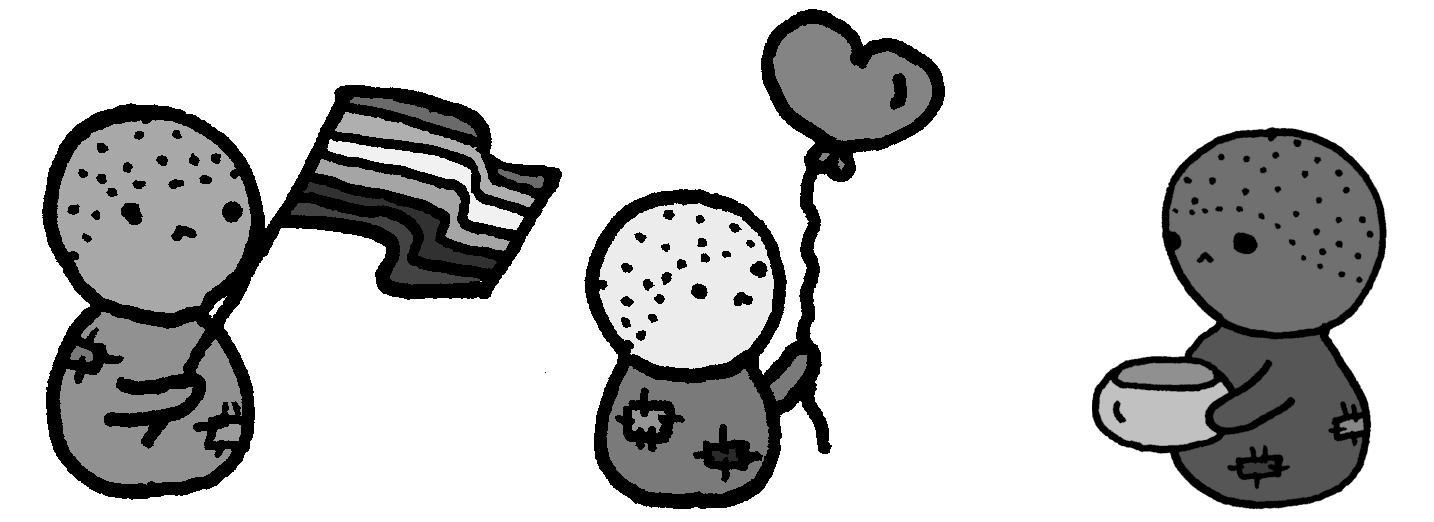
\includegraphics[width=0.7\paperwidth]{13bw.png}}
\end{figure}

\newpage
\thispagestyle{empty}
\begin{figure}[h]
    \centering
    \makebox[0pt]{%
    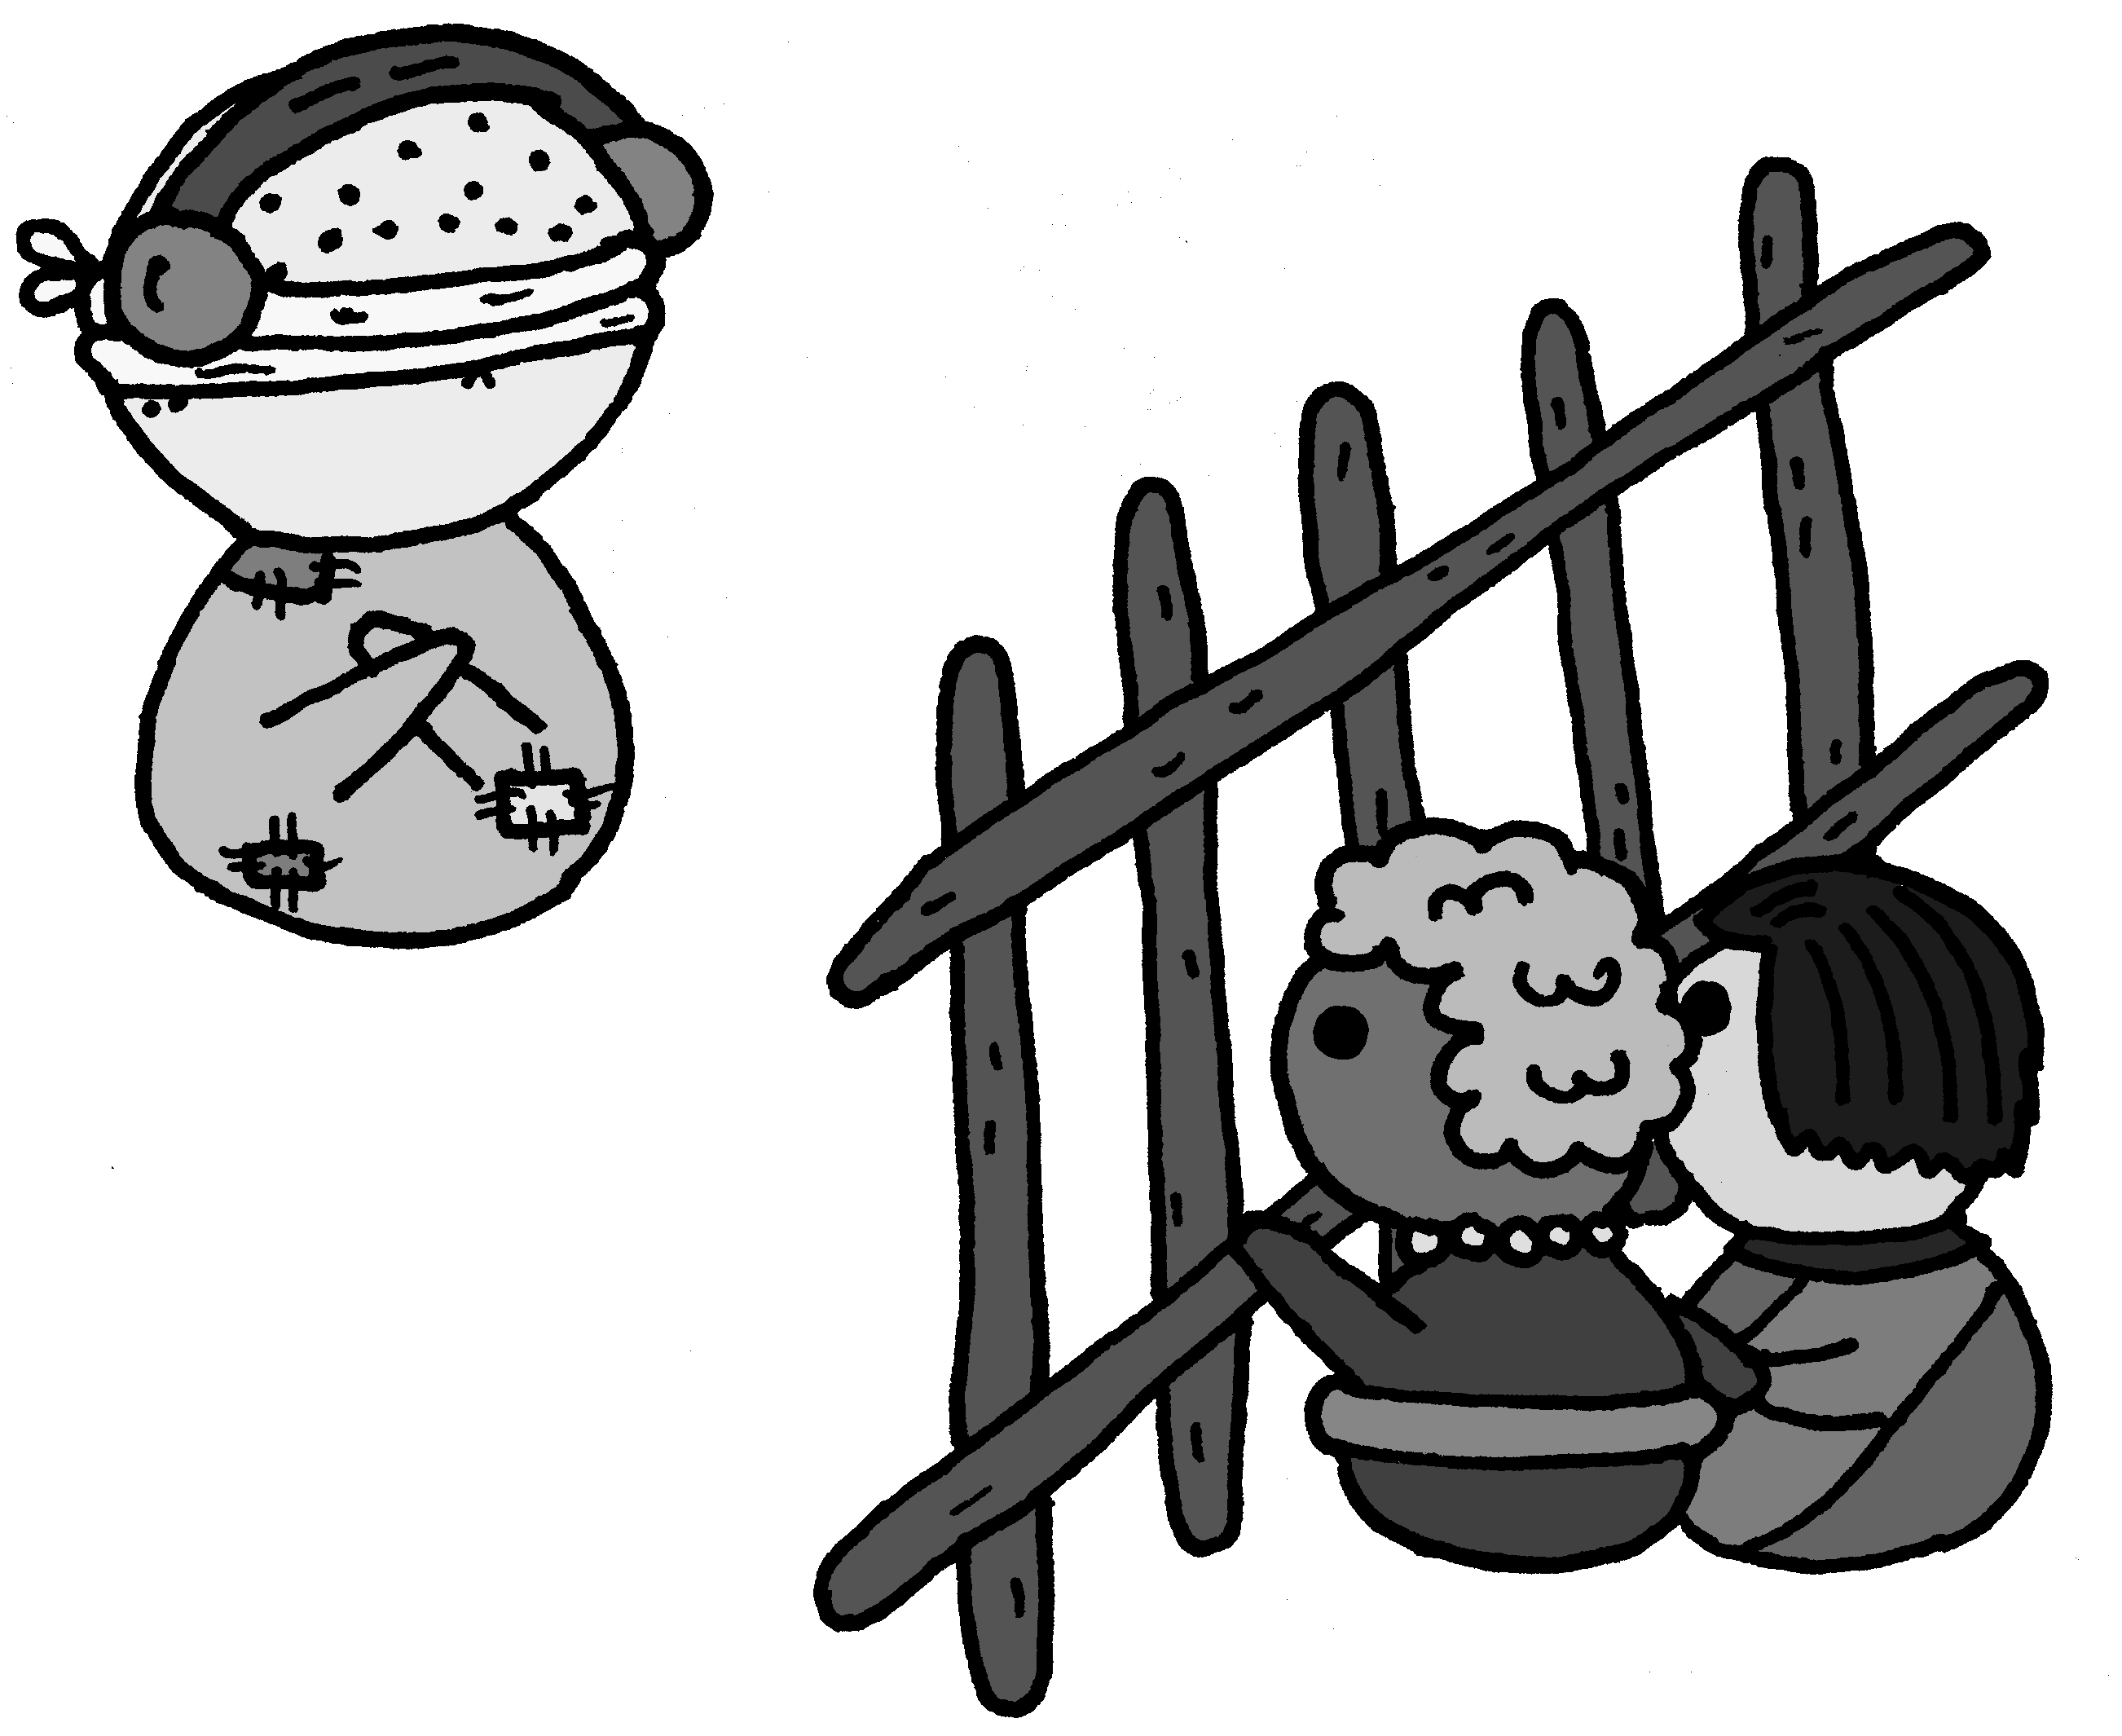
\includegraphics[width=0.8\paperwidth]{14bw.png}}
\end{figure}

\begin{quote}
\centering
\textit{\Large Hetzij boeddhistische individuen en organisaties actief inclusief zijn, zullen LGBTQIA+’ers nog steeds uitgesloten worden.}
\end{quote}

\chapter*{Obstakels voor LGBTQIA+ inclusie}
\addcontentsline{toc}{chapter}{Obstakels voor LGBTQIA+ inclusie}
\markboth{Verwelkom de regenboog}{Obstakels voor LGBTQIA+ inclusie}

\begin{wrapfigure}{r}{0.2\textwidth}
    \centering
    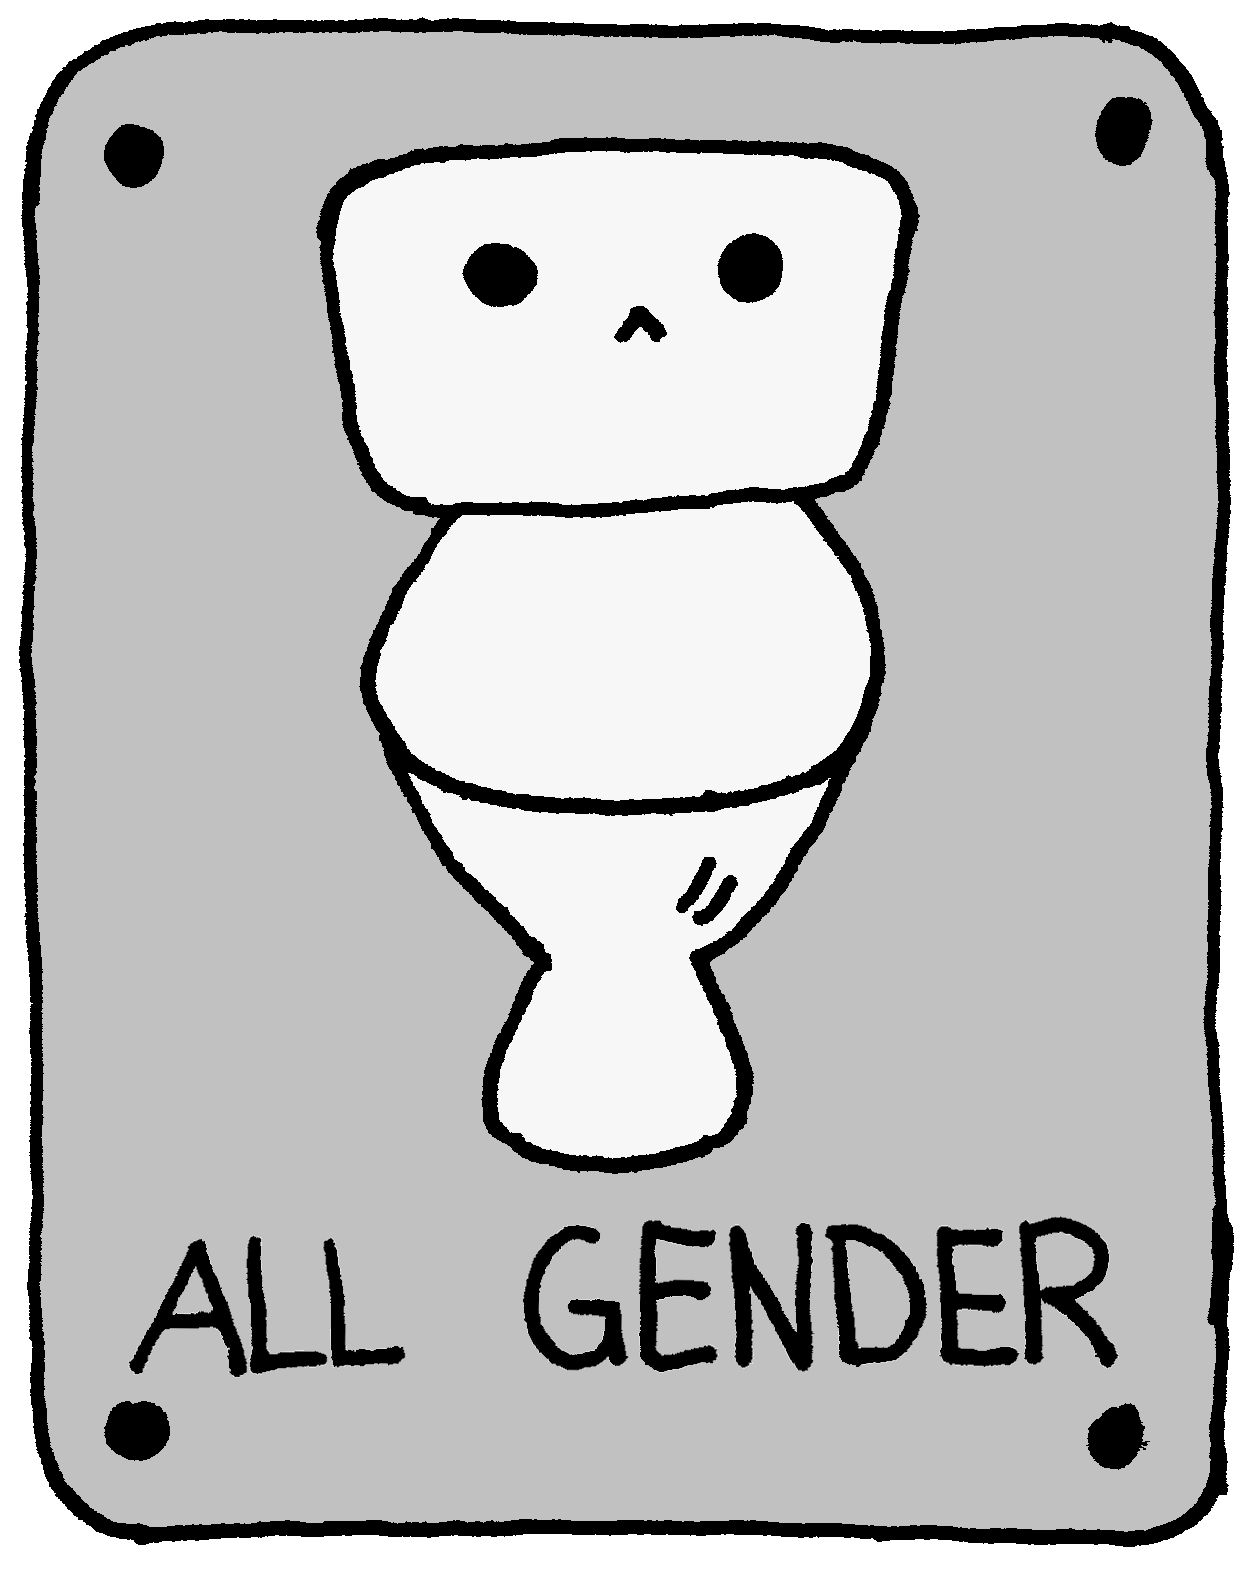
\includegraphics[width=0.2\textwidth]{16bw.png}
\end{wrapfigure}
De opzet en exploitatie van boeddhistische organisaties kan van grote invloed zijn op het buitensluiten van LGBTQIA+’ers. Een analogie: fysieke obstakels, zoals trappen, kunnen rolstoelgebruikers uitsluiten, dus hebben gebouwen hellingen en liften om ze binnen te laten. Op dezelfde manier zijn er administratieve, fysieke en conceptuele drempels die LGBTQIA+’ers uitsluiten. Mogelijk zijn we ons niet eens bewust van deze obstakels, maar ze bestaan en hebben werkelijke gevolgen.

\begin{quote}
\textit{We kunnen helpen om obstakels weg te nemen die \mbox{LGBTQIA+’ers} uitsluiten, en zo veiligere en meer inclusieve boeddhistische gemeenschappen creeren.}
\end{quote}

\phantomsection
\section*{Administratieve obstakels die uitsluiten}
\addcontentsline{toc}{section}{Administratieve obstakels die uitsluiten}

Op registratieformulieren en online databases kan vaak alleen uit mannelijke of vrouwelijke opties gekozen worden.  Dit sluit veel transgender, niet-binaire en ook sommige intersekse mensen uit die zich liever identificeren als “noch man noch vrouw”. Het hebben van alleen binaire opties geeft deze mensen al voordat ze zich voor een retraite of nieuwsbrief hebben opgegeven het idee dat ze vergeten zijn of niet welkom.

Het is meer inclusief om een optie ‘overig’ toe te voegen aan formulieren waarin naar geslacht wordt gevraagd. Dus behalve een “dhr”, “mevr”, ook een optie “mx” of “n.v.t.” of “anders”. De naam en het gender die sommigen in het dagelijks leven gebruiken is soms niet hetzelfde als wat in de officiele papieren staat vermeld. Voeg opties toe voor de roepnaam en vraag welke voornaamwoorden ze het liefst gebruiken. Overweeg ook of het wel nodig is om gender en aanhef te weten. Op sommige formulieren is deze informatie namelijk niet ter zake doende en nutteloos.

\phantomsection
\section*{Fysieke obstakels die uitsluiten}
\addcontentsline{toc}{section}{Fysieke obstakels die uitsluiten}

\subsubsection*{Gender-gescheiden zitplaatsen}

Sommige boeddhistische centra hebben gendergebonden zitgebieden in meditatiezalen, eetzalen en andere ruimtes. Soms kan dit zelfs een hierarchische indeling zijn, met vrouwen die achter mannen zitten. Gender-gescheiden openbare ruimtes werken simpelweg niet voor iedereen en kunnen een veilig gevoel ontnemen. 

Sommige transmensen krijgen door een gendergerelateerde ruimte ongewenst de aandacht op zich gevestigd en voelen hierdoor een angst om afgewezen te worden. Het kan stress opleveren voor non-binaire mensen als ze gedwongen worden om een beslissing te nemen over de plek waar ze zouden moeten gaan zitten, zeker als hun gender niet onmiddellijk herkenbaar is. Andere mensen houden niet van gendersegregatie omdat ze het ouderwets en onnodig vinden.

\subsubsection*{Toiletten}

Het moet mogelijk zijn om een toilet te kiezen die past bij je genderidentiteit. Sommige transgender en non-binaire mensen gaan liever naar een toilet voor “alle genders”, “iedereen” dan het heren- of damestoilet. Als er op het boeddhistische centrum of op andere retraite lokaties een toilet is voor iedereen helpt dat om genderdiverse mensen zich veilig en geaccepteerd te laten voelen.

\subsubsection*{Retreat accomodatie}

Iedereen zou zich welkom en veilig moeten kunnen voelen tijdens een retraite, maar voor veel LGBTQIA+’ers kan huisvesting een bron van ellende zijn. Er kunnen zorgen zijn over afwijzing vanwege hun seksuele geaardheid of buitengesloten worden vanwege hun gender of ze kunnen het gevoel hebben dat er simpelweg geen rekening wordt gehouden met hun behoeften. 

Alle mensen, of ze nou cisgender of transgender of non-binair zijn, zouden de mogelijkheid moeten krijgen om een accommodatie te kiezen die het beste bij hun genderidentiteit past.  Aangezien in veel retraite-centra de accommodaties in mannen- en vrouwenafdelingen verdeeld zijn is het belangrijk dat organisaties zich houden aan wettelijke verplichtingen met betrekking tot discriminatie van transgender mensen bij het gebruik van de accommodatie.

Hoewel er altijd behoefte zal blijven aan accomodatie voor specifieke genders, bevestigt dat voor veel transgender en non-binaire mensen niet het bestaan van andere genderidentiteiten, of dat sommige mensen zich niet identificeren als mannelijk of vrouwelijk. Door meer slaapzalen aan te bieden is het retraitecentrum meer inclusief en biedt het meer veilige alternatieven: vrouwenzalen, mannenzalen, gemengde zalen. Door op het inschrijfformulier deze opties op te sommen kunnen mensen kiezen wat hen het beste past.

Sommige mensen van hetzelfde gender willen wellicht naar een slaapzaal voor alle genders omdat een verblijf in een slaapzaal van hetzelfde geslacht een te grote uitdaging kan zijn. Kamergenoten kunnen er namelijk voor zorgen dat ze zich niet welkom voelen omdat ze queer zijn, of er kan afleiding ontstaan door verlangens.

Een extra slaapzaal voor “alle genders” geeft trans, non-binaire en gays een extra keuze om dat te kiezen wat voor hen het beste is. Een andere mogelijkheid is dat LGBTQIA+ers een eenpersoonskamer als voorkeur kunnen opgeven om de retraite-ervaring zo comfortabel mogelijk te laten zijn. 

Het verwelkomen van LGBTQIA+’ers begint dus lang voordat ze op de retraitelokatie aankomen. Je kunt dit bijvoorbeeld op de volgende manieren doen:

\begin{itemize}
  \setlength\itemsep{0em}
  \item Zorg dat op de publicaties staat dat het een veilige en inclusieve ruimte is voor LGBTQIA+’ers.
  \item Maak registratieformulieren met opties voor verschillende genders, voornaamwoorden en accomodatievoorkeuren.
  \item Zorg dat retraitemanagers en vrijwilligers zich bewust zijn van inclusieve omgang met LGBTQIA+’s.
  \item Zorg voor “alle gender” toiletten en bied meerdere accommodaite-opties.
  \item Herinner iedereen tijdens de orientatiesessie aan het begin van de retraite eraan dat het een inclusieve en gastvrije ruimte is voor iedereen, inclusief LGBTQIA+’ers.
\end{itemize}

\begin{figure}[h]
    \centering
    \makebox[0pt]{%
    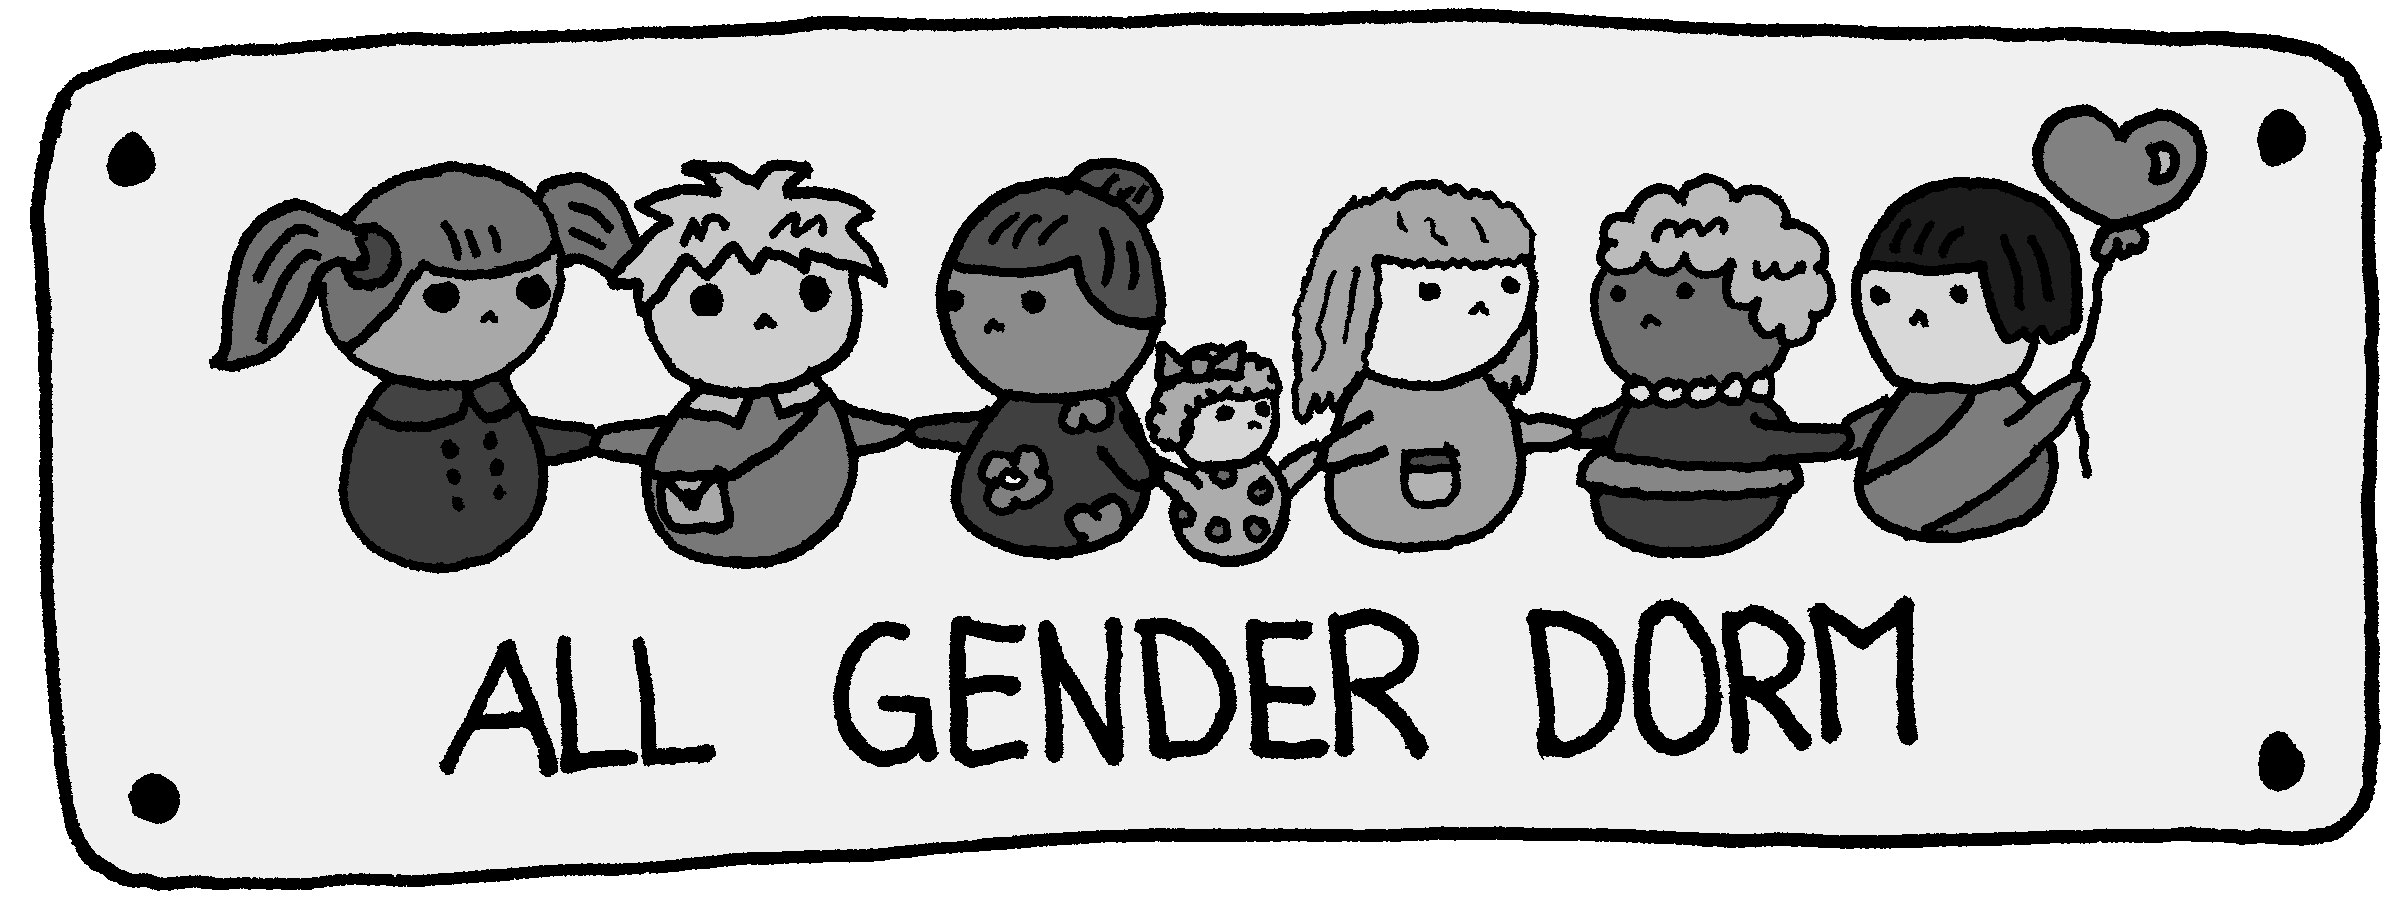
\includegraphics[width=0.6\paperwidth]{18-19bw.png}}
\end{figure}

\newpage
\thispagestyle{empty}
\begin{figure}[h]
    \centering
    \makebox[0pt]{%
    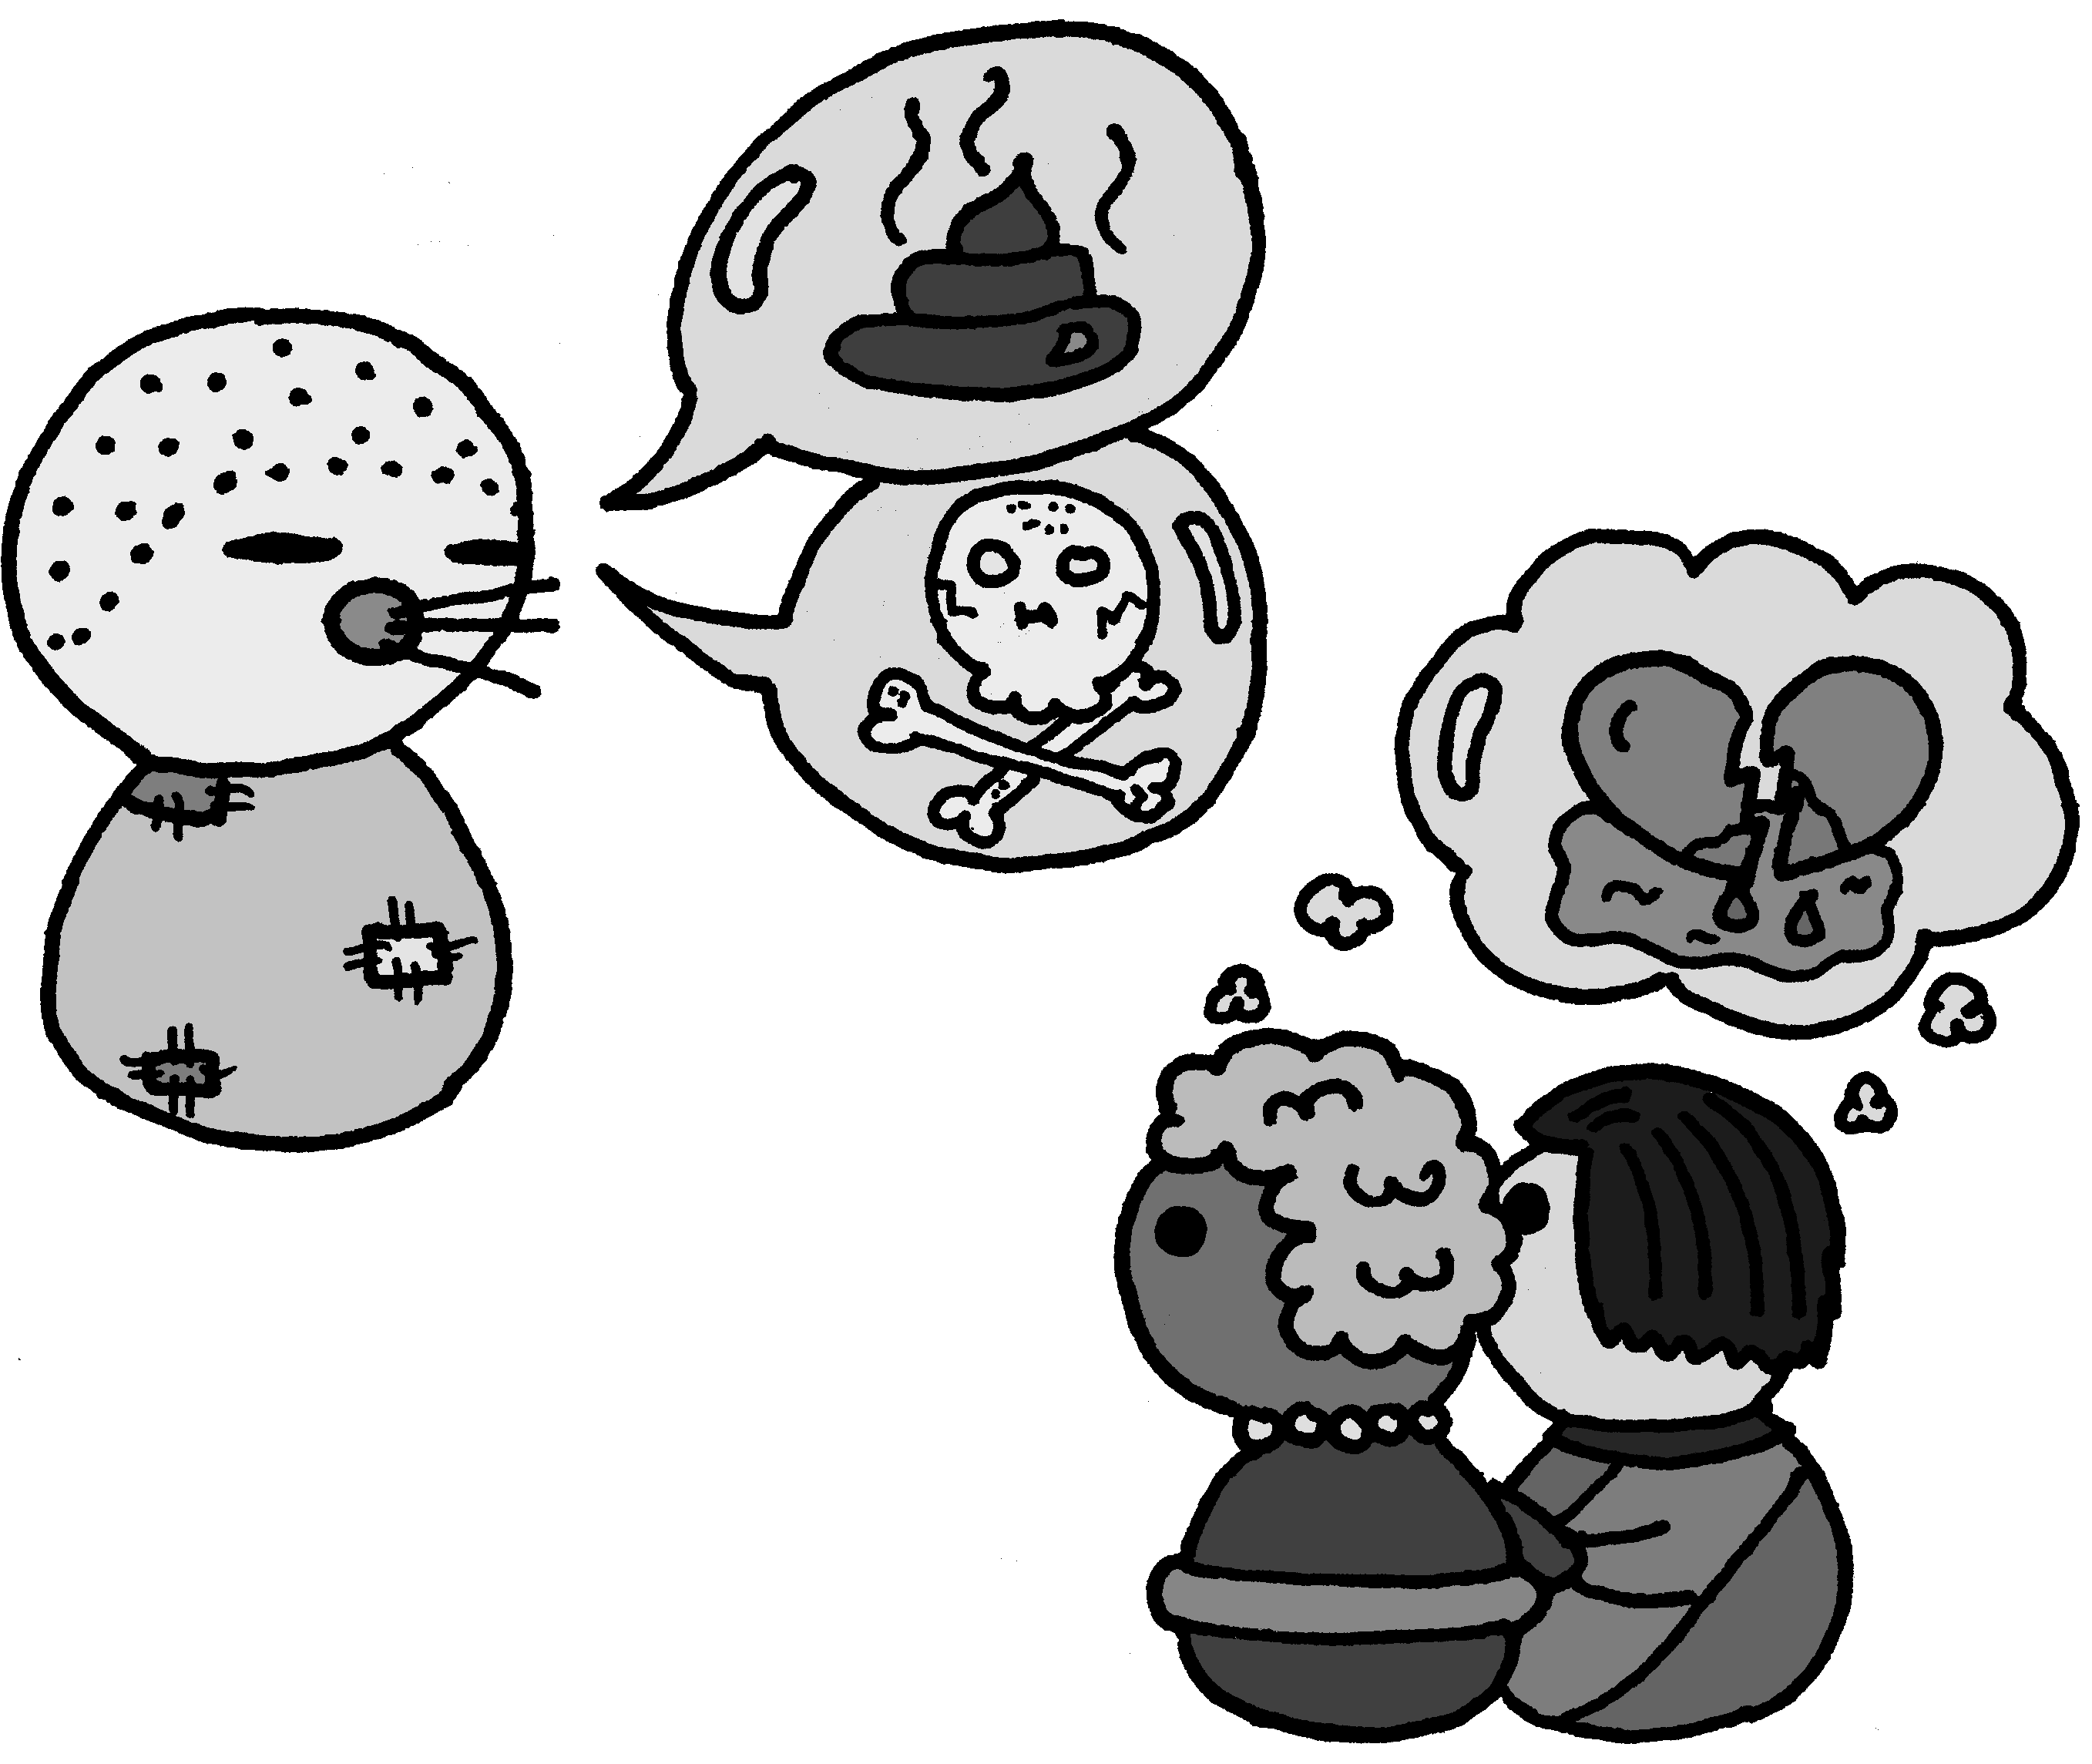
\includegraphics[width=0.8\paperwidth]{20bw.png}}
\end{figure}

\begin{quote}
\centering
\textit{\Large Ons taalgebruik kan mensen zich veilig, gerespecteerd en geaccepteerd laten voelen. Woorden kunnen mensen ook van streek maken, beledigen en buitensluiten.}
\end{quote}

\chapter*{Kwetsend taalgebruik}
\addcontentsline{toc}{chapter}{Kwetsend taalgebruik}
\markboth{Verwelkom de regenboog}{Kwetsend taalgebruik}

\phantomsection
\section*{Woorden die pijn doen}
\addcontentsline{toc}{section}{Woorden die pijn doen}

“Juist spreken” is een belangrijk boeddhistisch concept. Onze woorden hebben consequenties. Vriendelijke woorden veroorzaken geen schade en daarmee tonen we respect. Woorden kunnen mensen ook kwetsen en het gevoel geven niet welkom te zijn. Respectloos taalgebruik, flauwe grappen en indringende vragen stroken niet met juist spreken en kunnen het moeilijk maken voor LGBTQIA+’ers om een onderdeel te zijn van boeddhistische organisaties.

Hieronder een aantal belangrijke tips bij het spreken met en over LGBTQIA+’ers.

\subsubsection*{Respectvol taalgebruik}

Wees altijd vriendelijk en gebruik bewust geen woorden die als kwetsend kunnen worden opgevat. Aanstootgevende taal kan ook ernstige juridische gevolgen hebben.

\begin{itemize}
  \setlength\itemsep{0em}
  \item Vermijd verouderde termen als homoseksueel, transseksueel, travestie en hermafrodiet. Deze woorden hebben medische connotaties die LGBTQIA+’ers kunnen stigmatiseren.
  \item Gebruik geen aanstootgevende woorden als homo, tranny, sissy, lady-boy, hij-zij, manwijf of ‘het’.
  \item Vermijd zinnen die denigrerend zijn zoals ‘dat is zo gay’ of ‘no homo’.
\end{itemize}

\subsubsection*{Taal die uitsluit}

Bewust omgaan met taal is een goede manier om van boeddhistische gemeenschappen een plek te maken waar iedereen zich thuis voelt.  Hier zijn wat tips:

\begin{itemize}
  \setlength\itemsep{0em}
  \item Vermijd binaire taal die trans en non-binaire mensen uitsluit. Zeg in plaats van ‘dames en heren’ of ‘broeders en zusters’ gewoon: ‘hallo allemaal’ of ‘beste mensen’.
  \item Vermijd gender exclusieve taal. Zeg eens ‘de gemiddelde persoon op straat’ in plaats van ’de gemiddelde man op straat’. En in plaats van ‘jongens’ kun je ‘mensen’ zeggen.
  \item Wees je bewust van het uitsluiten van mensen die op hetzelfde geslacht vallen. Zeg in plaats van ‘echtgenoten en echtgenotes’ gewoon ‘partners’. In plaats van het te hebben over ‘aantrekking tot het andere geslacht’ kun je het beter gewoon ‘aantrekking’ zeggen.
\item Reduceer niemand op basis van hun lichaamsdelen of seksuele geaardheid. Onthoud dat iedereen een volwaardig persoon is en meer dan de som van deze zaken. Omschrijf iemand niet op basis van hun seksualiteit (“die homo daar”) of met hun medische geschiedenis (“die omgebouwde daar” of “zij is man-naar-vrouw”).
\end{itemize}

\begin{quote}
\textit{Inclusieve taal maakt dat mensen zich welkom voelen, uitsluitende taal sluit mensen buiten}
\end{quote}

\subsubsection*{Ongepaste vragen}

In een openbare setting indringende vragen stellen over iemands persoonlijke leven is altijd ongepast. Iemand ondervragen over hun geslachtsdelen, chirurgische ingrepen, seksuele geaardheid of hun seksleven is ongewenst omdat deze zaken voor iedereen erg privé zijn. Ongepaste vragen zijn onder andere: 

\begin{itemize}
  \setlength\itemsep{0em}
  \item Ben je een jongen of een meisje / man of vrouw?
  \item Heb je je een (geslachtsveranderende) operatie ondergaan?
  \item Hoe heette je voor de transitie?
  \item Wie is het mannetje in jullie relatie?
  \item Welke houding vind je leuk in bed?
  \item Ben je wel eens naar bed geweest met iemand van het andere geslacht?
  \item Maar als je bi bent, waarom ben je dan getrouwd?
\end{itemize}

\subsubsection*{Dubbelzinnige complimenten}

Iemand een compliment geven omdat hij op een heteroseksueel of cisgender lijkt is beledigend omdat het klinkt alsof dat op de een of andere manier beter zou zijn dan LGBTQIA+. Deze ideeen zijn ook gebaseerd op stereotypen en erkennen de werkelijke diversiteit in de Maatschappij niet. Dubbelzinnige complimenten zijn onder andere: 

\begin{itemize}
  \setlength\itemsep{0em}
  \item Je komt helemaal niet gay op me over!
  \item Ik had niet kunnen raden dat je trans bent.
  \item Je bent behoorlijk gespierd voor een gay man.
  \item Je ziet er niet lesbisch uit.
\end{itemize}

\subsubsection*{Ongepaste grappen} 

Iets kan grappig klinken voor de een en kwetsend voor een ander. Grappen over gender, seksualiteit of over het lichaam zijn Meestal niet grappig voor LGBTQIA+ mensen omdat ze vaak bedoeld zijn om ze buiten te sluiten, te pesten en belachelijk te maken. 

\subsubsection*{Seksuele toespelingen}

Gebaren en seksuele opmerkingen over het geslacht, seksualiteit of het lichaam is in gezelschap ongepast.

\subsubsection*{Stereotypering}

Stereotypering geeft mensen het gevoel dat ze niet als individu worden gezien. Vergeet niet dat de LGBTQIA+-gemeenschappen uit zeer diverse groepen bestaan en dat mensen binnen elke groep ook weer onderling verschillen. Ze houden niet allemaal van dezelfde dingen en hebben ieder hun eigen interesses. 

\subsubsection*{Outing}

Onthul niet zonder toestemming iemands seksuele voorkeur of gendergeschiedenis. Roddelen over dat soort dingen kan mensen kwetsen en valt onder “onjuist spreken”.

\phantomsection
\section*{Het belang van voornaamwoorden}
\addcontentsline{toc}{section}{Het belang van voornaamwoorden}

We vinden het allemaal belangrijk om te worden erkend en gerespecteerd om wie we zijn.

Voornaamwoorden verwijzen naar mensen, zoals ‘jij’, ‘wij’ en ‘hen’. Voornaamwoorden beschrijven ook het gender van mensen, zoals ‘zij’, ‘haar’ en ‘hun’ Het correct gebruik van voornaamwoorden is altijd waardevol en respectvol. We vinden het allemaal prettig als mensen ons aanspreken met de voornaamwoorden die bij ons passen. Dit geldt ook voor trans- en gender-diverse mensen. 

Voornaamwoorden maken deel uit van iemands identiteit, net zoals een naam dat doet. Het voornaamwoord dat iemand gebruikt om zichzelf te omschrijven weerspiegelt over het algemeen de genderidentiteit. Gender is een spectrum. Hoe mensen zich soms identificeren lijkt niet altijd te kloppen met hun uiterlijk of stemgeluid, dus mogen we er niet vanuit gaan dat iemands voornaamwoord gebaseerd is op iemands uiterlijk en stemgeluid. Het is beter om bij iemand op diskrete wijze te informeren, en vervolgens hun voornaamwoorden te gebruiken in gesprekken met die persoon of met andere mensen.

\noindent\fbox{%
    \parbox{\textwidth}{%
\textit{\textbf{\Large ‘Zij/hun/(van) hen’ voornaamwoorden}}

\medskip

In het Engels wordt ‘they/them/their’ gebruikt als een enkele persoon wordt bedoeld waarvan gegenderde voornaamwoorden nog onbekend zijn. Deze genderneutrale voornaamwoorden hebben een gebruiksgeschiedenis die teruggaat naar het jaar 1375. In het Nederlands kun je ‘diegene’ of ‘die persoon’, of ‘hun/hen’ zeggen. Genderneutraal is ook: ‘Iemand heeft hier een paraplu achtergelaten’. ‘Hoe kunnen we erachter komen van wie de paraplu is?’ Of ‘Ik weet niet zeker welke voornaamwoorden ik zou moeten gebruiken. Ik zal het diegene de volgende keer vragen’.
    }%
}

\subsubsection*{Soorten voornaamwoorden}

De gebruikelijke voornaamwoorden zijn: ‘zij/haar/(van) haar’ en ‘hij/ hem/(van) hem’. Sommige mensen hebben een identiteit die buiten de mannelijke/vrouwelijke binaire valt en zij gebruiken genderneutrale voornaamwoorden, zoals ‘die/hun/(van) hen’. Andere mensen zullen ‘hij’ en ‘zij’ afwisselend gebruiken om aan te geven dat hun gender fluide is. Sommige mensen geven er de voorkeur aan om alleen met hun voornaam genoemd te worden.

\subsubsection*{Voornaamwoorden correct gebruiken}

We kunnen in boeddhistische centra het goede voorbeeld geven door inclusieve woorden te gebruiken. Zo maken we duidelijk dat het gebruik van de juiste voornaamwoorden belangrijk wordt gevonden. Als we dat doen zullen trans en genderdiverse mensen zich meer welkom, begrepen en geaccepteerd voelen.

\begin{itemize}
\setlength\itemsep{0em}
\item Stel jezelf voor met je voornaamwoorden; ‘Hoi, ik ben Bodhi. Ik gebruik ’zij/haar’ voornaamwoorden’. 
\item Vraag beleefd en discreet welk voornaamwoord anderen gebruiken. ‘Hoi ik ben Lotus. Ik gebruik ’zij/haar’ voornaamwoorden. Hoe zal ik jou aanspreken?’ 
\item Gebruik altijd de naam en het voornaamwoord dat ze zelf nu gebruiken, ook als je het over hun verleden hebt.
\item Corrigeer anderen in je gemeenschap als ze iemand verkeerd hebben aangesproken of een verkeerde naam hebben gegeven. Zo help je hen het belang van een correct gebruik van voornaamwoorden in te laten zien.
\item Voeg je eigen voornaamwoorden en naam toe aan je e-mail handtekening, visitekaartje, docentenprofiel of biografie; bijvoorbeeld Mitra Lovegood (zij/haar), boekhoudafdeling.
\end{itemize}

Onthoud dat niet iedereen zijn voornaamwoorden wil delen en dat niemand daartoe gedwongen zou moeten worden. 

\phantomsection
\section*{Misgenderen}
\addcontentsline{toc}{section}{Misgenderen}

Misgenderen is iemand omschrijven of aanspreken met woorden die niet passen bij hoe die persoon zich met eigen gender of lichaam indentificeert. 
Het is elementaire beleefdheid om iemand op de gewenste manier aan te spreken. Misgenderd worden voelt onwaardig, afkeurend en respectloos. Het geeft mensen het gevoel er niet bij te horen. 

Door simpelweg iemand te vragen naar hun voornaamwoorden toon je respect voor hun genderidentiteit. Totdat je zeker bent welk voornaamwoord iemand gebruikt kun je die persoon genderneutraal aanspreken. Als het gender bekend is gebruik je het geprefereerde voornaamwoord. Zodra iemand zich voorstelt als vrouw of man laat je het neutrale voornaamwoord weer vallen.

Het is niet erg als je het fout doet. Iedereen vergist zich wel eens. Bied je excuses aan na gebruik van het verkeerde voornaamwoord, zeg het goede voornaamwoord en stap er overheen zonder er een probleem van te maken. Als je pas later bedenkt dat je je hebt vergist, neem dan even de desbetreffende persoon apart, verontschuldig je en ga weer over tot de orde van de dag.

\subsubsection*{Verkeerde naamgeving}

Namen zijn belangrijk voor ons allemaal. Het is beleefd om iemands naam correct te gebruiken. Verkeerde naamgeving (ook wel ‘dead-naming’ genoemd) is het verwijzen naar een trans persoon met de naam die gebruikt werd voor de transitie. Dit kan kwetsend en storend zijn voor transgender mensen. Vraag nooit aan iemand om hun oude naam te onthullen. Als iemand heeft besloten om de identiteit te bevestigen met een nieuwe naam is het wel zo attent om die naam ook te gebruiken. Dat is respectvol en biedt steun. 

\phantomsection
\section*{Ongemakkelijke instructies}
\addcontentsline{toc}{section}{Ongemakkelijke instructies}

Het is prettig wanneer meditatieleraren zich ervan bewust zijn dat sommige trans mensen zich erg ongemakkelijk voelen over hun lichaam. Dit wordt ook wel ‘genderdysforie’ genoemd. Het is een hoogst ongemakkelijk gevoel door incongruentie tussen het geslacht dat ze bij geboorte kregen en hun genderidentiteit. Mocht iemand die mediteert last hebben van genderdysforie, bied dan meditatietechnieken aan die zich niet op de ongemakkelijke lichaamsdelen gericht zijn. Dus wanneer iemand worstelt met dysforie op de borst, stel dan loopmeditatie voor of metta-meditatie of iets anders wat niet de aandacht vestigt op de borst.

Tijdens een meditatiegroep is het een goed idee om meerdere meditatietechnieken aan te bieden. Dit is vooral belangrijk voor een beginnersgroep aangezien die nog niet hebben leren omgaan met ongemakkelijke sensaties of emoties.

Degene die een retraite groep leidt kan ook in hun taalgebruik rekening houden met mensen met verschillende lichamen, genderidentiteiten en seksuele geaardheden en zou er niet vanuit moeten gaan dat iedereen in de retraite heteroseksueel of cisgender is.



\chapter*{Kwetsende meningen}
\addcontentsline{toc}{chapter}{Kwetsende meningen}
\markboth{Verwelkom de regenboog}{Kwetsende meningen}

\phantomsection
\section*{De pijnlijke realiteit van discriminatie}
\addcontentsline{toc}{section}{De pijnlijke realiteit van discriminatie}

\begin{quote}
\textit{De opvattingen van mensen kunnen leiden tot vooroordelen en onverdraagzaamheid, discriminatie en onderdrukking, alsmede haat en geweld tegen LGBTQIA+ gemeenschappen.}
\end{quote}

Ondanks dat de meeste LGBTQIA+’ers een gezond en gelukkig leven leiden, blijkt uit onderzoek dat een onevenredig aantal van hen het zwaar heeft qua geestelijke gezondheid en een hoger risico op suicidaal gedrag vertoont. Dit is direct gerelateerd aan ervaringen met stigma, vooroordelen, discriminatie en misbruik vanwege het LGBTQIA+ zijn. 

LGBTQIA+’ers worden over de hele wereld gepest, verbaal misbruikt en hebben te maken met geweldadige aanvallen. Deze pijnlijke feiten maken duidelijk hoe belangrijk het is om te blijven praten over discriminatie en vooroordelen, zodat er begrip komt voor de uitdagingen waar LGBTQIA+’ers tegen aanlopen, en we ruimtes kunnen creëren waar alle mensen zich gastvrij en welkom voelen.

\noindent\fbox{%
   \parbox{\textwidth}{%
\textit{\textbf{\Large Discriminatie van LGBTQIA+’ers}}

\begin{itemize}
\setlength\itemsep{0em}
\item 72 landen zien consensuele seksuele handelingen tussen mannen als een misdaad.
\item 44 landen zien  consensuele seksuele handelingen tussen vrouwen als een misdaad.
\item 11 landen geven de doodstraf voor consensuele seks met hetzelfde geslacht.
\item 15 landen zien gender identiteit van transgender mensen als een misdaad en hebben wetten m.b.t. ‘travestie’, ‘imitatie’ en ‘vermomming’.
\item Over de hele wereld zijn er intersekse mensen die lijden onder gedwongen medische ingrepen die hun mensenrechten en lichamelijke integriteit schenden.
\end{itemize}
   }
}

\phantomsection
\section*{Een opmerking over niet-zelf}
\addcontentsline{toc}{section}{Een opmerking over niet-zelf}

Sommige boeddhisten beschuldigen LGBTQIA+’ers er ten onrechte van dat ze geobsedeerd zijn door hun identiteit of het vasthouden aan een idee van ‘zelf’. Ze wijzen op de boeddhistische leer van \textit{anatta} (niet-zelf) en houden vol dat identiteit slechts een illusie is en dus niet bestaat. Ook wordt beweerd dat het focussen op een identiteit in strijd is met de boeddhistische leer en dat dit de oorzaak is van het lijden van LGBTQIA+’ers. 

Het is echter belangrijk om te bedenken dat het zijn van queer, trans of intersekse een fundamenteel onderdeel is van het menszijn. Suggereren dat deze aspecten van een persoon op de één of andere manier onecht of onbelangrijk zijn is onjuist en misbruik van de boeddhistische leer. Het ontkent de waarheid van de ervaringen die iemand heeft doorgemaakt en wist belangrijke delen van hun leven uit, zoals relaties, gemeenschappen of werk. Deze mening is eveneens schadelijk omdat het de bestaande discriminatie, vooroordelen en het geweld dat LGBTQIA+’ers elke dag ervaren deels ontkent. 

Sommige boeddhisten gebruiken het ‘niet-zelf’-concept om LGBTQIA+’ers de mond te snoeren en de zeer reëele pijn die ze voelen zo te ontkennen. LGBTQIA+’ers lijden vooral onder de houding die sommigen hebben ten aanzien van hun identiteit. LGBTQIA+ zijn is op zichzelf geen oorzaak van lijden net zo min als cisgender of heteroseksueel zijn dat is. LGBTQIA+’ers hebben het over identiteit omdat ze vaak sociaal beïnvloed worden door mensen met een discriminerende houding en ze willen veranderingen aanbrengen in de delen van de samenleving die schade aanrichten. Gender en seksualiteit zijn een belangrijk onderdeel van het menszijn en van de maatschappij. De diversiteit mag op handen worden gedragen in plaats van genegeerd of uitgewist worden. 

Daarom is het echt belangrijk dat boeddhisten nadenken over hoe er over ‘niet-zelf’ wordt gesproken met mensen die onderdrukt worden naar aanleiding van hun identiteit. Anders wordt het ‘niet-zelf’, in plaats van een nuttig hulpmiddel voor persoonlijke groei, een wapen dat anderen beschadigt. Deze ‘bewapende \textit{anatta}’ kan aanvoelen als de zoveelste oneerlijke aanval op LGBTQIA+’ers.  

\subsubsection*{Wie ben je?}

LGBTQIA+’ers ontvangen soms kritiek wanneer ze dingen willen bespreken die hen aangaan, en krijgen dan te horen dat ze geobsedeerd zijn met hun identiteit. Als er over ‘niet-zelf’ wordt gesproken is het van belang om in te zien dat heteroseksuele mensen en cisgenders ook een gender hebben en een seksuele identiteit. Dat inzicht is mogelijk niet vanzelfsprekend omdat die groepen zichzelf als normaal zien. De maatschappij bekrachtigt die identiteit waardoor het vaak niet eens opvalt.

We kunnen ons afvragen:

\begin{itemize}
\setlength\itemsep{0em}
\item Vink ik op formulieren altijd hetzelfde vakje aan voor mijn gender?
\item Zou het me irriteren als iemand me met het verkeerde gender aanspreekt?
\item Zou ik iemand corrigeren als ze mij met een verkeerde naam of titel aanspreken?
\end{itemize}

Als je hier positief op antwoordt betekent dit dan dat je geobsedeerd bent met je identiteit?

Of we kunnen empathie ontwikkelen door eens na te denken over:

\begin{itemize}
\setlength\itemsep{0em}
\item Hoe zou het voelen als mijn relatie door de regering strafbaar werd gesteld?
\item Wat als ik mijn baan kon verliezen door mijn geaardheid of gender?
\item Ben ik wel eens bang geweest voor een geweldadige aanval als ik iemand in het openbaar genegenheid wilde tonen?
\item Zou ik strijden voor gelijke rechten als ik zo behandeld zou worden?
\end{itemize}

Los van hoe ‘zelf’ en ‘niet-zelf’ wordt gezien, worden LGBTQIA+’ers wereldwijd gediscrimineerd en onderdrukt. Deze zaken zijn persoonlijk, sociaal en spiritueel. Zodra discussies over LGBTQIA+ binnen de boeddhistische gemeenschappen komen stil te liggen houdt dat de onderdrukking in stand.

Vergeet niet dat er aspecten aan het ‘zelf’ zijn waar boeddhisten zich juist mee vereenzelvigen, zoals vrijgevigheid, ethisch gedrag, vriendelijkheid, mededogen en wijsheid. LGBTQIA+’ers hebben deze kwaliteiten ook.

\phantomsection
\section*{Intersectionele identiteiten: ras, gender en seksualiteit}
\addcontentsline{toc}{section}{Intersectionele identiteiten: ras, gender en seksualiteit}

LGBTQIA+’ers ervaren racisme, klassisme, validisme en andere vooroordelen. De term “intersectionele identiteiten” omschrijft een raamwerk waarbinnen duidelijk wordt hoe een combinatie van verschillende identiteiten in gemeenschappen discriminatie en privileges in de hand werken. Dat gaat onder andere over ras, gender, seksualiteit, bekwaamheid, rijkdom, opleiding en locatie. Zo heeft een zwarte transvrouw in een westers boeddhistisch centrum een heel andere ervaring dan een heteroseksuele blanke cis-gender man in datzelfde centrum. Of een Aziatische gay cis-man kan in een klooster een heel andere ervaring hebben dan een witte heteroseksuele cis-vrouw op diezelfde plek.

Als we zien hoe identiteiten elkaar overlappen maakt dat ons bewust hoe discriminatie en privileges elkaar kruisen en enorm verschillende ervaringen creëren, zelfs voor mensen die gedeeltelijk dezelfde identiteiten hebben. Het is daarom van cruciaal belang dat deze verschillen begrepen worden omdat het laat zien dat de ervaringen van mensen uit dezelfde samenleving niet allemaal hetzelfde zijn, en dat er dus verschillende benaderingen nodig zijn om inclusie en gelijkheid voor verschillende groepen in onze gemeenschappen te bevorderen.

\begin{quote}
\textit{Het is belangrijk om te erkennen dat we niet allemaal hetzelfde zijn en te begrijpen dat onze verschillen ertoe doen}
\end{quote}

\begin{figure}[h]
    \centering
    \makebox[0pt]{%
    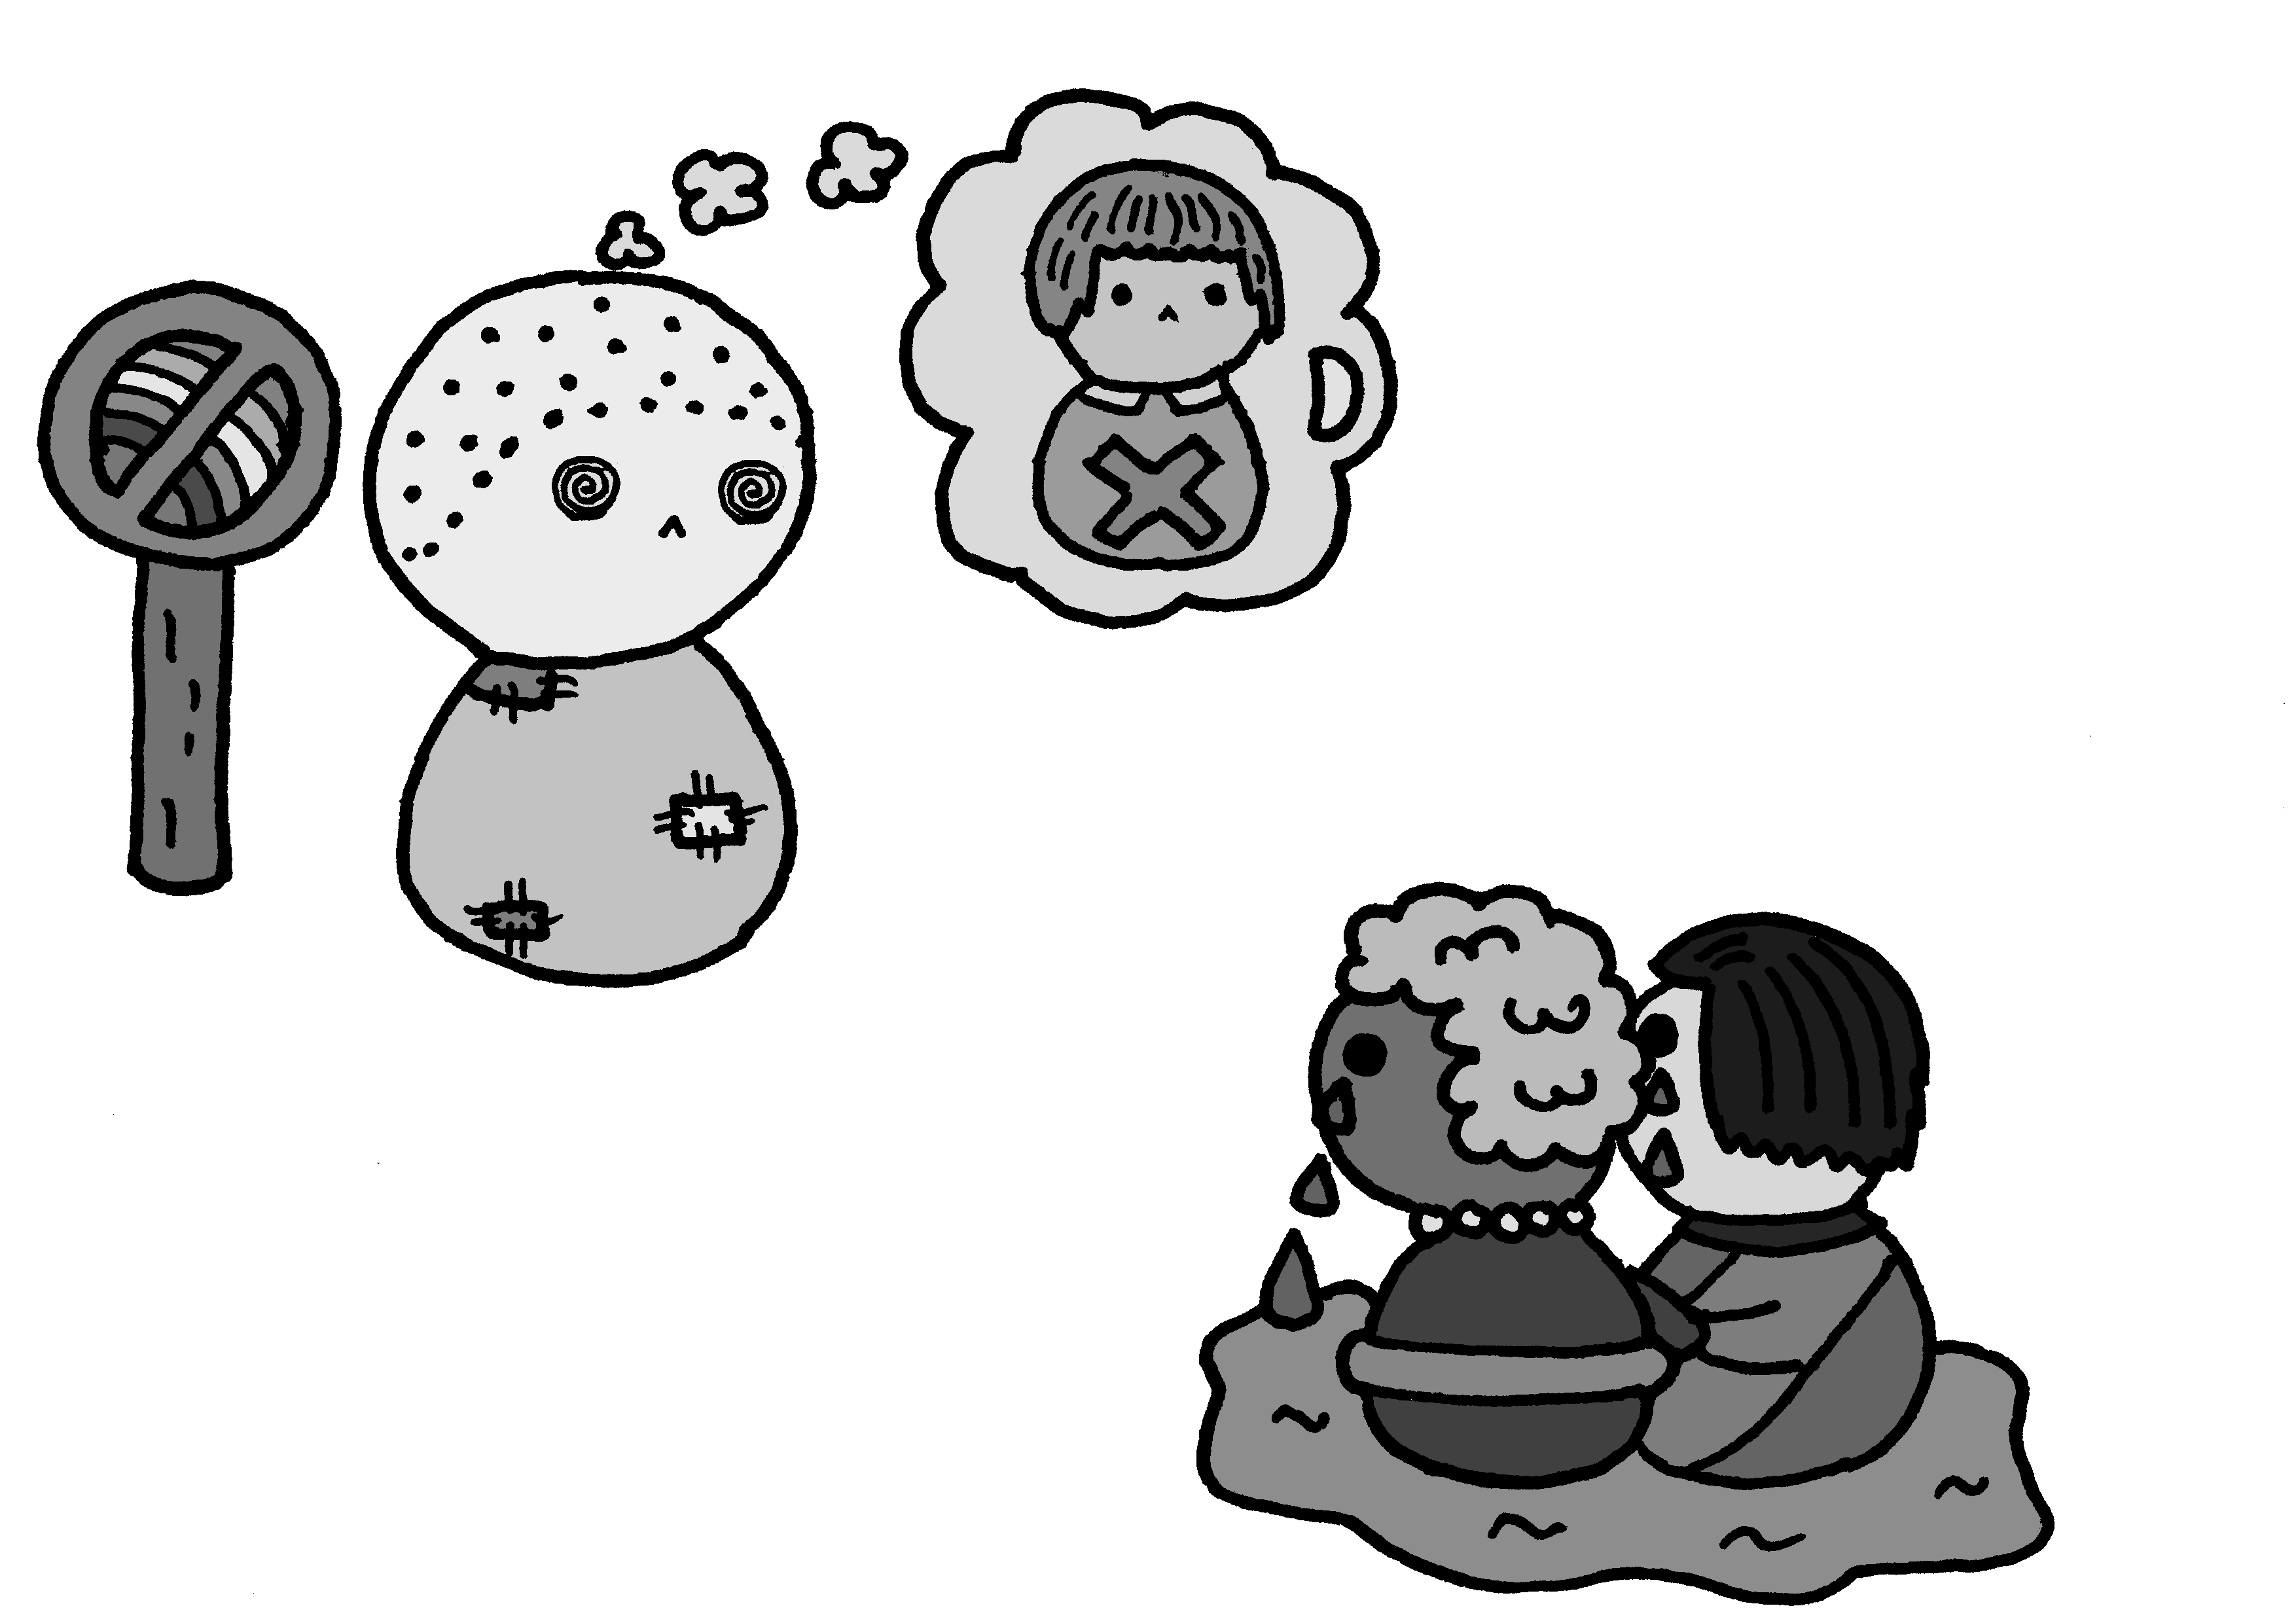
\includegraphics[width=0.4\paperwidth]{30bw.png}}
\end{figure}

\chapter*{Een LGBTQIA+’ers gids}
\addcontentsline{toc}{chapter}{Een LGBTQIA+’ers gids}
\markboth{Verwelkom de regenboog}{Een LGBTQIA+’ers gids}

\begin{quote}
\textit{LGBTQIA+ gemeenschappen zijn zeer divers. Ze omvatten individuen, relaties, families, vriendschappen, subculturen en nog veel meer!}
\end{quote}

\phantomsection
\section*{Het verschil tussen lichaam, gender identiteit en seksualiteit}
\addcontentsline{toc}{section}{Het verschil tussen lichaam, gender identiteit en seksualiteit}

Iedereen heeft een lichaam, gender identiteit en seksualiteit. Het is belangrijk om deze basisbegrippen en terminologieën enigzins te kennen om inzicht te krijgen in de zaken waar de LGBTQIA+ gemeenschap mee te maken heeft.

\subsubsection*{Lichaams- en geslachtskenmerken}

Elk lichaam is anders. Er zijn zoveel onderlinge verschillen in vorm en formaat en gelaatstrekken. Geslachtskenmerken verschillen onderling ook, zoals in fysieke kenmerken die horen bij lichaamsontwikkeling, hormoonregulatie en het voortplantingssysteem. Primaire geslachtskenmerken zijn geslachtsklieren, chromosomen, geslachtsorganen en hormonen. Secundaire geslachtskenmerken ontstaan in de puberteit en gaan over borstweefsel, stemhoogte, gezichts- en schaamhaar.

‘Geslachtskenmerken’ klinkt beter dan het ‘biologisch geslacht’ of termen als ‘biologisch mannelijk’ of ‘biologisch vrouwelijk’. Want lichaamsdelen op zich bepalen niet of je man of vrouw bent. Veel mensen hebben mogelijk geleerd dat er maar twee soorten lichamen zijn—mannelijk en vrouwelijk—maar eigenlijk bestaan er veel meer soorten lichamen.

\subsubsection*{Lichaam en gender}

Lichaam en gender zijn twee totaal verschillende dingen. Het hebben van een bepaald sort lichaam betekent niet dat daar een bepaald gender bij hoort. Het gender van een persoon staat los van welk lichaam of lichaamsdelen iemand heeft.

Genderidentiteit maakt deel uit van ons \textit{interne} zelfgevoel. Het gender kan vrouwelijk, mannelijk, geen van beiden, een combinatie van beiden, of weer iets heel anders zijn. De relatie die iemand met hun gender heeft kan ook veranderen in de loop van de tijd.

\subsubsection*{Toegewezen gender}

De meesten van ons krijgen bij geboorte een gender toegewezen dat tijdens het opgroeien wordt bevestigd door de mensen om ons heen. Veel mensen zijn het eens met het gender dat ze toegewezen kregen bij geboorte, maar sommigen niet.  

\subsubsection*{Cisgender}

Cisgender (kortweg “cis”) verwijst naar mensen die zich uitsluitend identificeren met het gender dat ze bij geboorte werd toegewezen. Als iemand bij geboorte voor jongen werd aangezien en zich identificeert als man is het een cis-man. ‘Cis’ is een Latijns word wat ‘aan dezelfde kant’ betekent. 

\begin{figure}[h]
    \centering
    \makebox[0pt]{%
    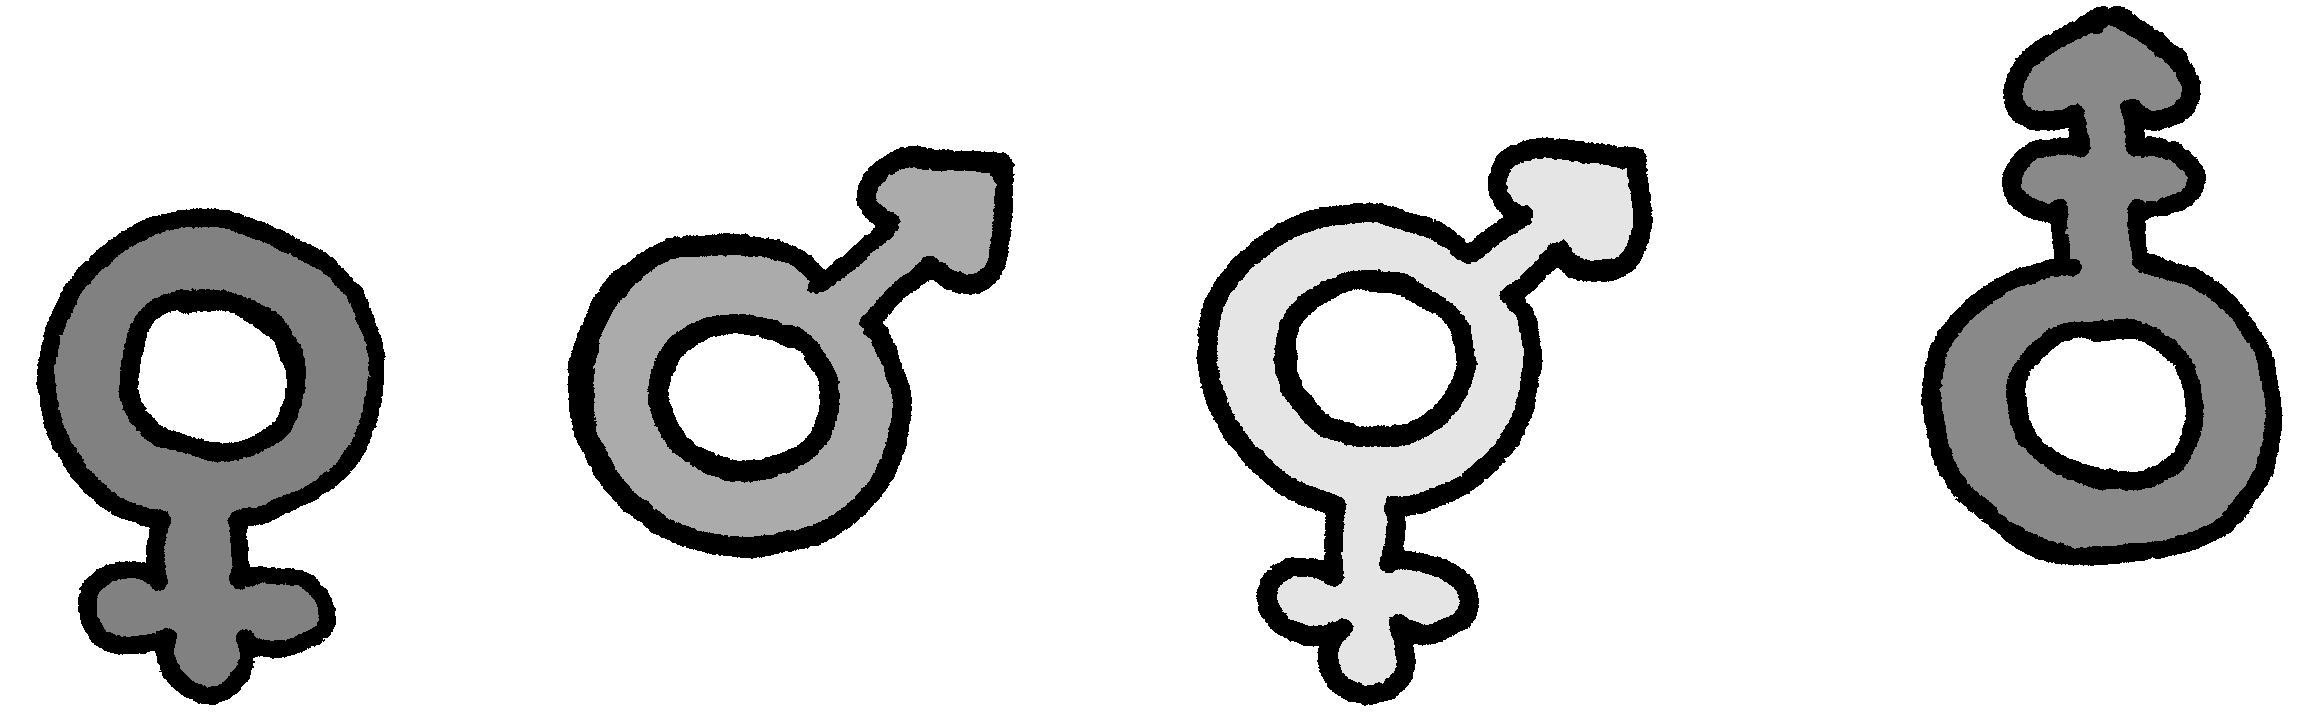
\includegraphics[width=0.4\paperwidth]{38-39bw.png}}
\end{figure}

\subsubsection*{Transgender} 

Transgender (kortweg “trans”) of gender-divers beschrijft mensen die zich niet uitsluitend identificeren met het gender dat ze bij geboorte kregen. Trans zijn gaat over genderidentiteit en wie we zijn, en gaat niet over welk gender we aantrekkelijk vinden.

\subsubsection*{Seksuele geaardheid} 

Seksuele geaardheid of seksualiteit geeft aan tot wie we ons wel of niet aangetrokken voelen. Seksuele geaardheid heeft niks te maken met het soort lichaam of geslachtskenmerken en het heeft ook niks te maken met gender of genderidentiteit. Seksualiteit is een spectrum en bij veel mensen verandert hun seksualiteit in de loop van hun leven.

\phantomsection
\section*{Intersekse}
\addcontentsline{toc}{section}{Intersekse}

Intersekse is een overkoepelende term die wordt gebruikt om mensen te omschrijven met natuurlijke variaties die afwijken van gangbare ideeën over ‘vrouwelijke’ of ‘mannelijke’ lichamen. Ongeveer 1,7\% van de mensen wordt geboren met intersekse kenmerken. Dat betreft een breed scala aan genitale, chromosomale, hormonale en andere fysieke kenmerken. Deze kenmerken kunnen prenataal al zichtbaar zijn of bij de geboorte pas zichtbaar worden, of zelfs pas zichtbaar worden rond de puberteit. Het kan ook nog later aan het licht komen, bijvoorbeeld bij het verwekken van een kind. Elke eigenschap heeft zijn eigen unieke kenmerken en uit zich in verschillende gradaties.

Veel intersekse mensen identificeren zich met het geslacht dat ze bij geboorte kregen toegewezen—simpelweg als man of vrouw. Anderen identificeren zich als “anders”. Sommige intersekse mensen verwerpen het geslacht dat ze bij geboorte kregen, maar zien zichzelf ook niet als transgender. Anderen identificeren zich als transgender of gender-divers.  

Intersekse mensen hebben net als niet-intersekse mensen een breed scala aan identiteiten. Sommigen willen bij de regenbooggemeenschap horen, anderen niet. Intersekse zijn gaat niet over genderidentiteit en is anders dan trans of non-binair zijn. Intersekse heeft ook niks te maken met seksuele geaardheid; intersekse mensen kunnen lesbisch, homoseksueel, biseksueel of heteroseksueel zijn net als ieder ander.

\noindent\fbox{%
    \parbox{\textwidth}{%
\textit{\textbf{\Large Houdingen die kwetsend zijn voor intersekse mensen}}

\begin{itemize}
\setlength\itemsep{0em}
\item Leven in een wereld die de lichamelijke anatomie van intersekse mensen niet erkent en deze mensen ook geen mensenrechten geeft.
\item Het verwijderen van geslachtskenmerken door niet-consensuele genitale chirurgie in de kindertijd en het toedienen van hormonen om intersekse kinderen een meer vrouwelijk of mannelijk uiterlijk te geven. 
\item Sociale schaamte en stigmatisering over het menselijk lichaam in het onderwijs, de gezondheidszorg, sport, werk en andere instellingen. 
\item Onjuiste en verouderde taal, zoals ‘hermafrodiet’, is misleidend en minachtend, of een intersekse variatie onterecht een ‘afwijking’ noemen, wat het niet is. 
\end{itemize}
    }%
}

\phantomsection
\section*{Trans en gender divers}
\addcontentsline{toc}{section}{Trans en gender divers}

Trans en gender divers zijn overkoepelende termen om mensen te omschrijven die zich anders identificeren dan het gender dat hen bij de geboorte werd toegewezen. Trans mensen kunnen hun transgender-zijn zien als een persoonlijk verhaal of ervaring in plaats van een identiteit op zich en beschouwen hun genderidentiteit als gewoon vrouwelijk, mannelijk of non-binair. Of ze kunnen zich specifiek identificeren als trans, transvrouw of transman.

De term ‘gender divers’ omvat allerlei verschillende manieren waarop gender ervaren kan worden. Iemand kan zich identificeren als transgender of twijfelen over het gender. Gender divers zijn eveneens mensen die zich noch als man noch als vrouw identificeren, zoals bij non-binaire mensen of bij degenen bij wie het gender meer een spectrum is. Termen die sommigen gebruiken om het spectrum van hun gender te omschrijven omvatten genderfluide, genderqueer en gender non-conform. 

\subsubsection*{Transitie of genderbevestiging}

Er is sprake van transitie of genderbevestiging zodra iemand stappen onderneemt om zich sociaal of fysiek meer in lijn met hun genderidentiteit te kunnen voelen. Het is een persoonlijk proces wat maakt dat je in de maatschappij kunt leven met het gender wat voor jouw gevoel klopt.

Er worden sociale, medische, chirurgische en juridische stappen ondernomen om het gender van een persoon te bevestigen. Transitie betekent niet dat iemand ‘van gender verandert’ of ‘een geslachtsverandering ondergaat’ of een man of vrouw ‘wordt’—nee, ze bevestigen het gender dat ze altijd al hadden. De reis van elke trans persoon is anders. Er bestaat niet een ‘volbrachte transitie’ en ieders transitie is op diens eigen manier compleet, los van uiterlijk, documenten, hormonen of chirurgie.  

Het process van transitie staat niet gelijk aan identificeren als trans. Sommige mensen die in transitie zijn kunnen zich identificeren als trans, maar anderen zullen zich simpelweg als man of vrouw identificeren.

\subsubsection*{Sociale transitie}

Dit is het proces waarbij een persoon hun genderexpressie verandert zodat dat beter klopt bij hun genderidentiteit. Het uit de kast komen als trans en het veranderen van uiterlijk, van naam en voornaamwoorden kan daar allemaal onderdeel van zijn. Mensen kunnen ook de manier waarop ze omgaan met gendergerelateerde ruimtes veranderen, zoals het veranderen van toiletgebruik. Deze sociale transitie kan ook door het wijzigen van geslacht op het paspoort, de geboorteakte en andere documenten.

\subsubsection*{Fysieke transitie}

De fysieke transitie gaat over het veranderen van uiterlijk, zoals kleding, make-up en kapsel, zodat dat pas bij de genderidentiteit. Er kan ook gekozen worden voor een medisch traject met hormonen of een mogelijke operatie.  

\subsubsection*{Non-binair}

‘Non-binair’, ‘NB’ of ‘enby’ is een onderdeel van de transparaplu. Non-binair is een term die wordt gebruikt voor mensen die zich niet identificeren als vrouw of man. Ze vinden dat hun gender zowel mannelijk als vrouwelijk is, of dat ze er ergens tussen in zitten of dat ze nog weer iets anders zijn. Non-binaire mensen kunnen wel een sterk gevoel van gender hebben. Het kan erg schrijnend zijn om te horen dat ze gedwongen worden om zich als man of vrouw te identificeren. Iemand kan zich uitsluitend identificeren als non-binair of zich verwant voelen met non-binair als overkoepelende term voor allerlei verschillende ervaringen horend bij het non-binaire gender. Termen onder deze paraplu zijn onder andere genderfluide, genderqueer (ervaren een gender-spectrum), trans-masculien en trans-feminien (non-binair maar meer naar één kant van het gender), a-gender (zonder gender) en bi-gender (identificeren zich als zowel man als vrouw). Deze en andere woorden beschrijven hoe NB mensen zich voelen over hun gender en hoe ze het tot uitdrukking brengen. Veel non-binaire mensen identificeren zich als transgender. 

Non-binair zijn is iets anders dan intersekse zijn. De meeste binaire mensen worden geboren met een lichaam dat er conventioneel mannelijk of vrouwelijk uitziet, maar groeien op met het gevoel anders te zijn. Non-binair zijn heeft niks te maken met seksuele geaardheid; een non-binair persoon kan net als anderen elke geaardheid hebben. Sommige non-binaire mensen kiezen ervoor om een operatie te ondergaan of hormonen in te nemen om hun lichaam zo te veranderen dat ze zich er meer in thuis gaan voelen. Anderen vinden dit onnodig en zijn tevreden met hun lichaam zoals het is. Sommige non-binaire mensen presenteren zich androgien terwijl anderen er gewoon conventioneel mannelijk of vrouwelijk uitzien, maar toch non-binair zijn.

\medskip

\noindent\fbox{%
    \parbox{\textwidth}{%
\textit{\textbf{\Large Houdingen die trans en non-binaire mensen kwetsen}}

\medskip

Cisseksisme/cisgenderisme is een discriminerende sociale mening die beweert dat de transgender ervaring niet bestaat. Deze pijnlijke opvatting houdt in dat alleen binaire identiteiten (mannelijk of vrouwelijk) waardevol of echt zijn en dat genderidentiteit vastligt bij geboorte en uitsluitend gebaseerd is op geslachtskenmerken. 

Misgenderen is het beschrijven of aanspreken van een persoon met behulp van woorden die niet overeenkomen met hun genderidentiteit. Dit gaat over onjuist gebruik van voornaamwoorden (zij, hij, hun), familietitels (vader, zus, oom) en andere woorden die van oudsher gegendered worden gebruikt, zoals stoer, schattig, enzovoort. 
  
Transfobie verwijst naar negatieve vooroordelen en stereotypen over trans en genderdiverse mensen. Transfobie omvat respectloos of beledigend taalgebruik en beperkt de manier waarop mensen hun gender mogen laten zien door middel van kleding, keuze van toiletgebruik of soort accomodatie. Transfobie omvat ook beledigende bedreigingen, fysiek geweld, seksuele initmidatie en uitsluiting van mensen vanwege de genderidentiteit.
    }%
}

\phantomsection
\section*{Seksuele orientatie}
\addcontentsline{toc}{section}{Seksuele orientatie}

Gender en seksualiteit zijn twee verschillende dingen. Gender is hoe we ons tot onszelf verhouden. Dit kan mannelijk zijn of vrouwelijk of nog iets anders. Seksualiteit is tot wie we ons aangetrokken voelen. Een cisgender persoon kan ook homoseksueel, heteroseksueel, biseksueel of aseksueel zijn. Een trans persoon kan ook heteroseksueel, biseksueel, aseksueel, homoseksueel of een andere seksualiteit hebben.

\subsubsection*{Lesbisch}

Iemand die zich identificeert als vrouw en zich seksueel en/of romantiesch aangetrokken voelt tot mensen die zich identificeren als vrouw.

\subsubsection*{Homoseksueel}

Iemand die zich identificeert als man en zich seksueel en/of romantisch aangetrokken voelt tot andere mensen die zich identificeren als man.

\subsubsection*{Queer}

Omschrijft allerlei seksuele orientaties en genderidentiteiten. Vroeger werd de term queer als denigrerend gebruikt maar tegenwoordig is de term queer teruggewonnen en wordt vaak gebruikt als een overkoepelende term om het volledige scala aan LGBRQIA+-identiteiten te beschrijven.  

\subsubsection*{Biseksueel}

Iemand die zich seksueel en/of romantisch aangetrokken voelt tot zowel mensen van hetzelfde gender als mensen van een ander gender. Biseksualiteit houdt niet per se in dat er maar twee genders zouden zijn, en de term panseksueel heeft zich ontwikkeld om specifiek een aantrekkingskracht te kunnen omschrijven die zich niet laat beperken door gender, inclusief de aantrekkingskracht tot trans en non-binaire mensen.

\subsubsection*{Heteroseksueel (Straight)}

Iemand die zich seksueel en/of romantisch aangetrokken voelt tot het tegenovergestelde geslacht.

\subsubsection*{Romantische orientatie}

Beschrijft tot wie we ons romantisch aangetrokken voelen. Dit kan los staan van onze seksuele geaardheid. Romantische orientaties werken op vrijwel dezelfde manier als seksuele orientaties en beschrijven de gender(s) waarin een persoon romantisch geintereseerd is.

\subsubsection*{Aseksueel/Ace}

Een seksuele geaardheid gedefinieerd door gebrek aan seksuele aantrekkingskracht, hetzij binnen een relatie of daarbuiten. Een aseksueel persoon kan nog steeds romantische aantrekkingskracht voelen over de breedte van het LGBTQIA+-spectrum en kan wel seksueel actief zijn maar doet dit zonder seksuele aantrekkingskracht te ervaren.

\bigskip

\noindent\fbox{%
    \parbox{\textwidth}{%
\textit{\textbf{\Large Houdingen die schade aanrichten aan mensen die op hetzelfde geslacht vallen}}

\bigskip

\textbf{Bifobie}: Een schadelijke houding ten opzichte van iemand die zich aangetrokken voelt tot meer dan een gender. Dit kan inhouden dat iemand wordt verteld dat hun seksualiteit ‘slechts een fase is’ of aangezet wordt om ‘een kant te kiezen’. Door een biseksueel als homoseksueel of heteroseksueel te bestempelen wanneer ze een bepaalde relatie hebben wist dat hun ware identiteit uit.

\medskip

\textbf{Heteronormativiteit}: De opvatting dat een heteroseksuele relatie de enige natuurlijke, normale en legitieme uiting van seksualiteit is en dat andere seksualiteiten of genderidentiteiten onnatuurlijk zijn en een bedreiging vormen voor de samenleving.

\medskip

\textbf{Homofobie}: Negatieve overtuigingen, vooroordelen en stereotypen over niet-heteroseksuele mensen. Verbale homofobie is een veelvoorkomende vorm, inclusief schelden, roddelen en beledigende woorden (‘flikker’ of ‘pot’) of zinnen als ‘dat is zo gay’. Bij homofobie horen ook beledigende bedreigingen, fysiek geweld, seksuele intimidatie, discriminerende wetgeving en het opzettelijk uitsluiten van iemand vanwege hun seksualiteit. 
    }%
}

\newpage
\textbf{Meer Informatie: }https://rainbodhi.org/resources/

\medskip

{\footnotesize
\begin{center}
\noindent \textbf{Oorspronkelijke uitgave 2021:} 
\\
This booklet was produced by LGBTQIA+ Buddhists. All identity groups in the rainbow acronym were consulted for input and feedback.

\noindent Many thanks to Venerable Vimala, Ayya Vimalanyani, Bhante Sumano, Erland Moeckli, JJ, Nilushi Disayanake, Letty, all the Rainbodhi crew, the Buddhist Council of NSW, GiveOUT Day Australia, Simone Ford, Bronwyn Sweeney and a special thanks to all the many people who donated funds to produce this booklet.
\medskip

\noindent First Published in Australia 2021
by MegaCity Books
for Rainbodhi LGBTQIA+ Buddhist Community
rainbodhi.org



\noindent

\includegraphics{by-nc-sa} \\
This work is created under a Creative Commons Attribution-NonCommercial-ShareAlike 4.0 International License \\
\medskip
\noindent A catalogue record for this book is available from the National Library of Australia. \\
\medskip
\noindent 978-0-64889593-1-1 \\
\medskip
Author: Akaliko Bhikkhu \\
Illustrator: Venerable Yodha \\
Contributor: Letty \\
Project management and design: Kerry Klinner, megacitydesign.com \\
Editor: Simone Ford \\
Proofreader: Bronwyn Sweeney

\bigskip

\textbf{Nederlandstalige uitgave 2022:}  \\
Vertaler: Anoniem \\
Proeflezer: Marein Könings \\
Illustratie omslag: Venerable Yodha \\
Formattering van de gedrukte uitgave: Remy Jakobson
\end{center}
}

\newgeometry{margin=0px}

\begin{figure}[ht]
    \centering
    \makebox[0pt]{%
    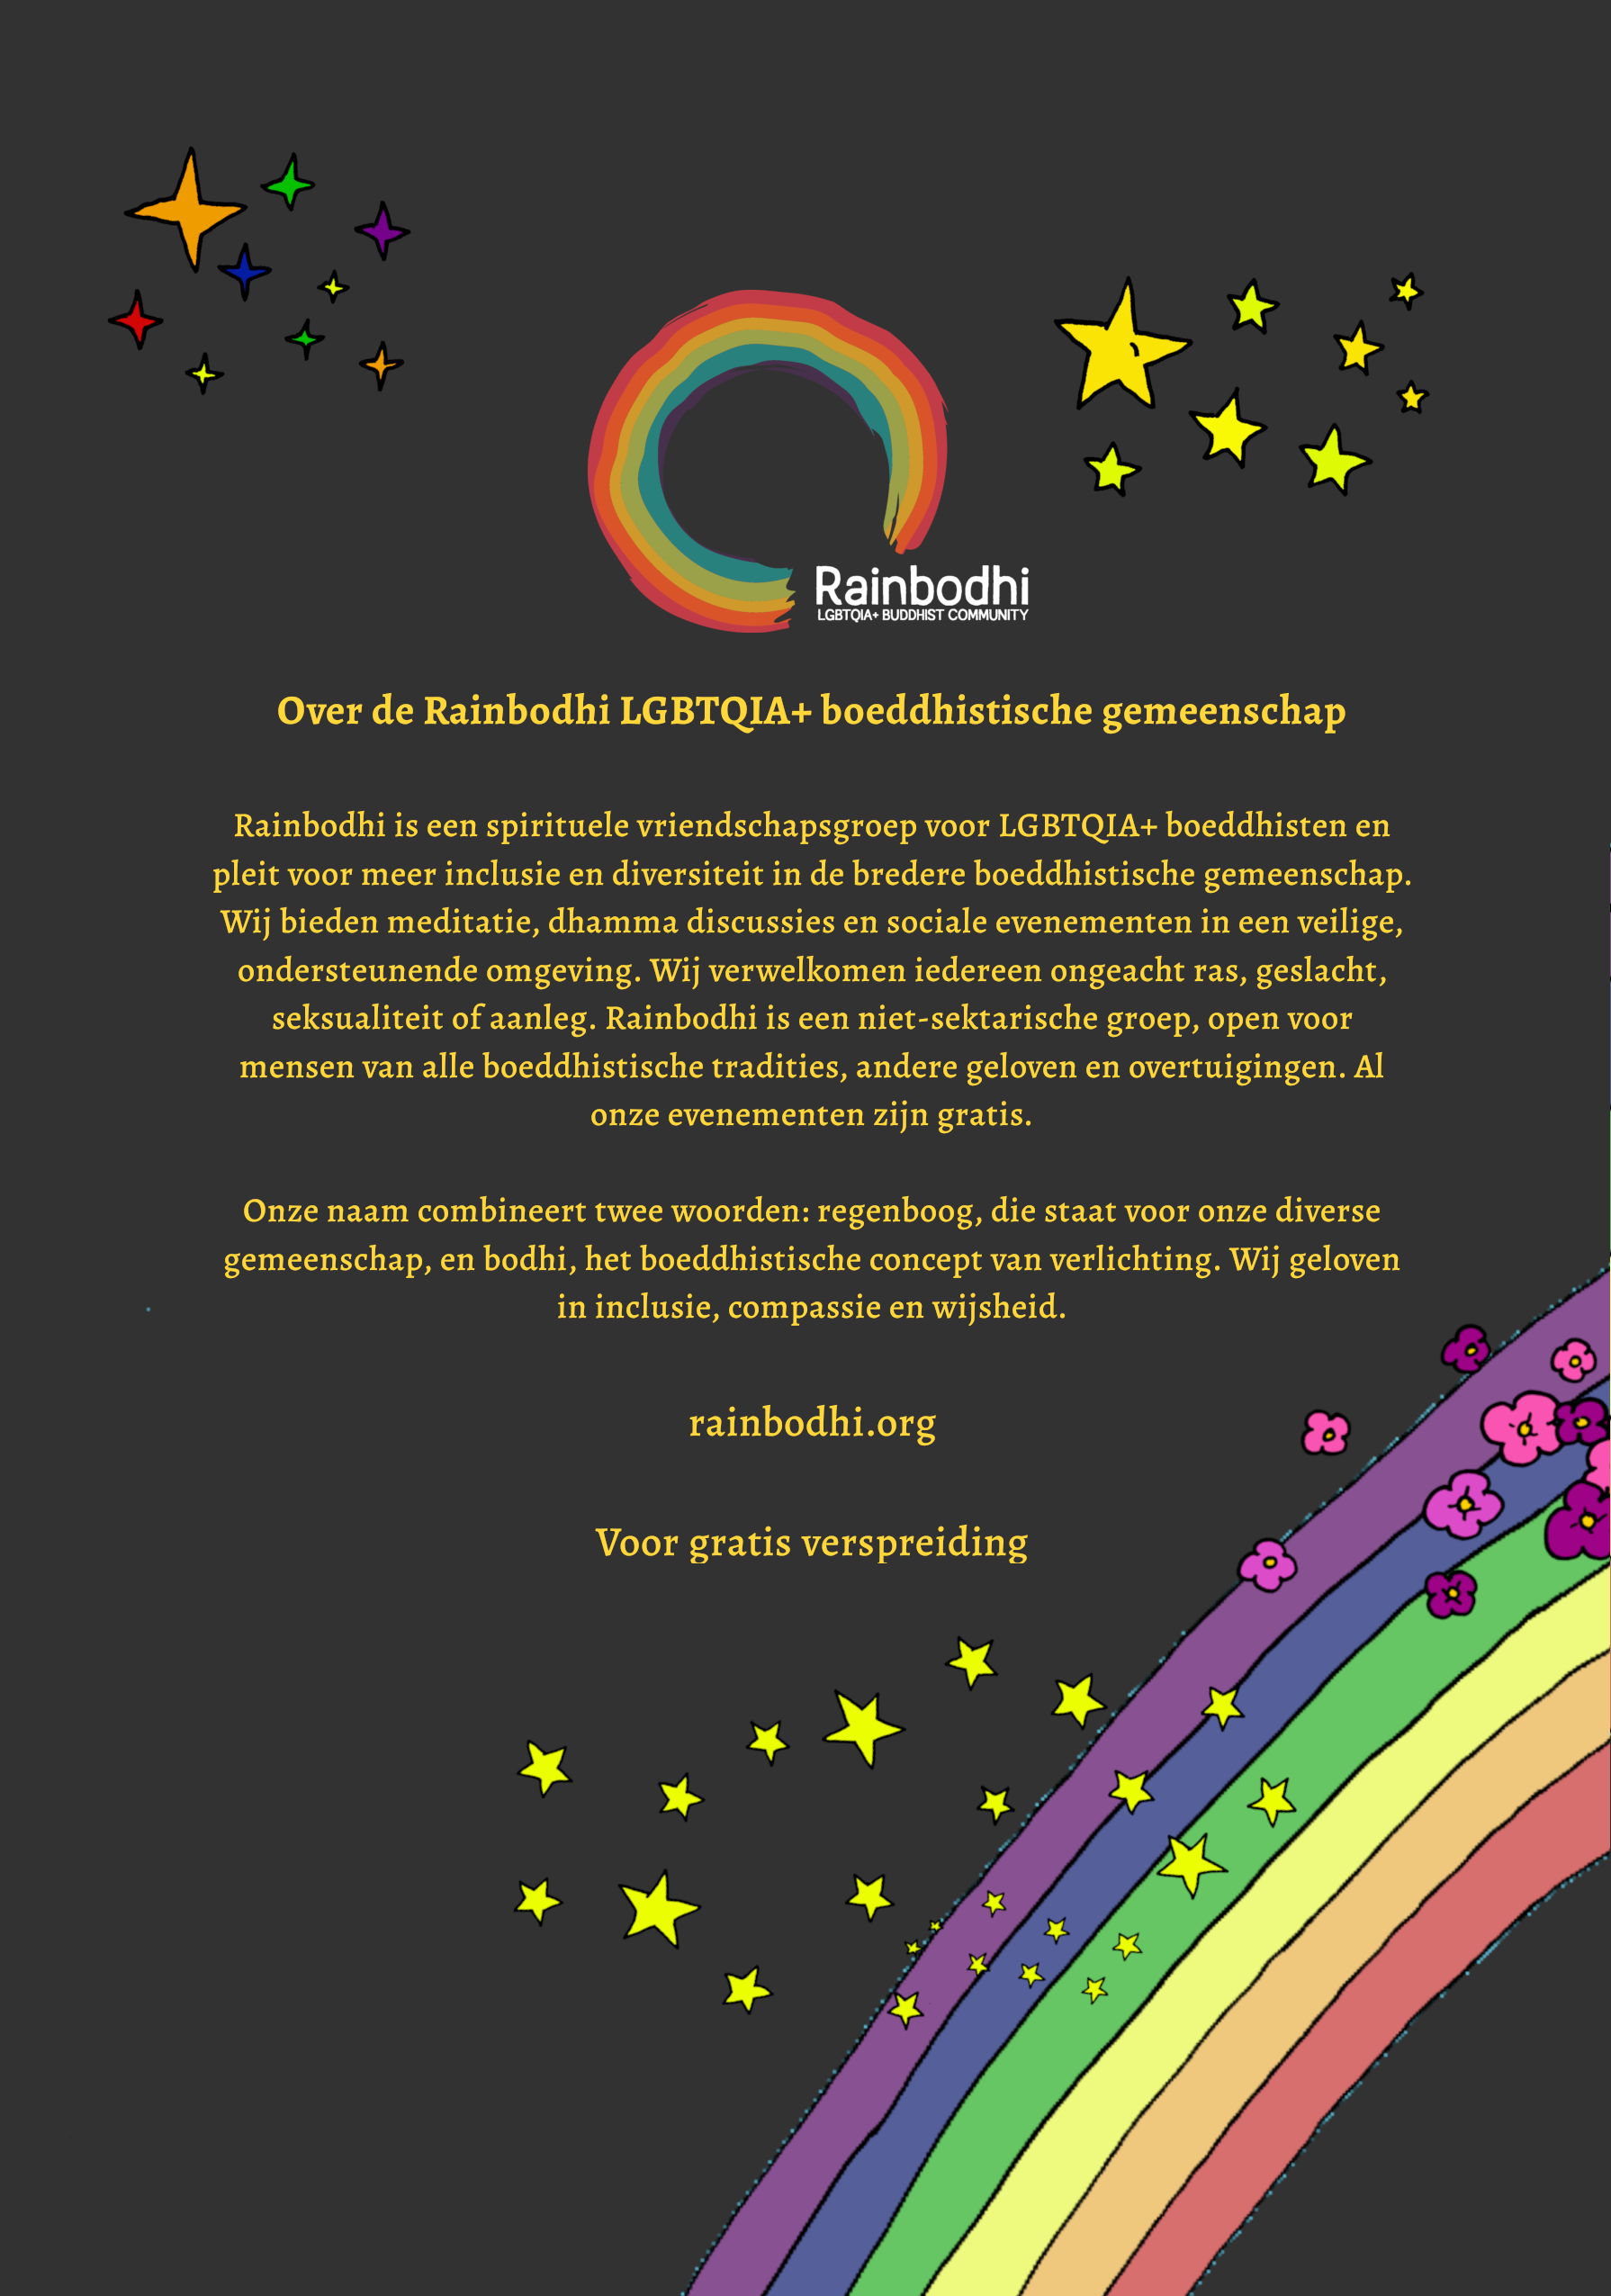
\includegraphics[width=\paperwidth]{back}}
\end{figure}

\end{document}

